\documentclass[a4paper,12pt,openright,notitlepage,twoside]{book}
\raggedbottom % lascia alla fine delle pagine lo spazio invece che adattarle


% pacchetti da caricare
\usepackage[T1]{fontenc} % definisce i caratteri di output
\usepackage[utf8]{inputenc} % definisce i caratteri di input
\usepackage[english]{babel} % definisce la lingua del documento
\usepackage[headheight=15pt]{geometry} % definisce i margini del documento
\geometry{a4paper,top=30mm,bottom=30mm,left=30mm,right=25mm,heightrounded,bindingoffset=3mm}
\usepackage{fancyhdr} % serve per gestire intestazione e piè di pagina
\pagestyle{fancy}
\usepackage{emptypage} % serve per fare le pagine vuote
\usepackage[pdftex]{hyperref} % serve per ottenere links e indice cliccabili
\hypersetup{colorlinks=true,allcolors=black}
\usepackage{microtype} % migliora la scrittura del testo
\usepackage{appendix} % serve per personalizzare l'appendice
\usepackage[printonlyused]{acronym} % serve per creare l'elenco degli acronimi
\usepackage{eurosym} % serve per scrivere il singolo dell'euro
\usepackage{siunitx} % serve per mettere le unita` di misura nel SI
\usepackage{mathtools} % serve per fare le formule matematiche (carica anche AMSMATH)
\usepackage{booktabs} % serve per fare le tabelle più belle
\usepackage{multirow} % serve per fare le tabelle con righe complesse
\usepackage{pgfplotstable} % serve per fare tabelle da file con dati tabulati
\usepackage{graphicx} % serve per fare le figure
\usepackage{tikz} % serve per fare i grafici
\usetikzlibrary{shapes}
\usepackage{pgfplots} % serve a fare i grafici anche lui
\pgfplotsset{compat=1.14}
\usepackage{subcaption} % serve per aggiungere la didascalia alle figure composte (carica anche CAPTION)
\captionsetup{font=small,labelsep=period,format=hang,tableposition=top,figureposition=bottom}
\usepackage{tocloft} % serve per fare le liste di figure e tabelle più belle
\usepackage{cite} % serve per mettere le citazioni bibliografiche
\usepackage{amsmath,amsfonts,amsthm,bm} % Math packages

\usepackage[ruled,vlined,linesnumbered]{algorithm2e}

\usepackage{soul}
\usepackage{color}

% modifiche dei comandi
\renewcommand{\chaptermark}[1]{\markboth{\chaptername\ \thechapter.\ #1}{}} % modifica l'intestazione con il nome/numero del capitolo
\renewcommand{\sectionmark}[1]{\markright{\thesection.\ #1}} % modifica l'intestazione con il nome/numero dela sezione
\renewcommand{\cftfigfont}{Figure } % per aggiungere "Figure " nella lista delle figure
\renewcommand{\cfttabfont}{Table } % per aggiungere "Table " nella lista delle tabelle


\DeclareMathOperator*{\argmin}{argmin} % thin space, limits underneath in displays


% Keywords command
\providecommand{\keywords}[1]
{
  \small	
  \textit{\textbf{Keywords---}} #1
}


% dichiarazioni personalizzate
\DeclarePairedDelimiter{\abs}{\lvert}{\rvert} % per fare il valore assoluto
\DeclarePairedDelimiter{\norma}{\lVert}{\rVert} % per fare la norma



\begin{document}

\frontmatter % serve per mettere i numeri romani come numeri di pagina 
\thispagestyle{empty} % serve per rimuovere tutte le impostazioni delle pagine dalla prima pagina

% FRONTESPIZIO
\begin{center}
% Intestazione
\Large{\textbf{Politecnico di Milano}} \\
\vspace{-4mm}
\rule{\textwidth}{0.4pt}
\normalsize{SCHOOL OF INDUSTRIAL AND INFORMATION ENGINEERING} \\
\normalsize{Master of Science -- Aerospace Engineering} \\
\vspace{20mm}
% Logo Politecnico
\begin{figure}[h!]
\centering
\includegraphics[height=0.15\textheight]{images/logo-polimi}
\end{figure}
\vspace{22mm}
% Titolo Tesi
\huge{\textbf{Thesis Title}} \\
\vspace{32mm}
\end{center}

% Relatore/Correlatore
\begin{flushleft}
\normalsize{Supervisor} \\
\small{\textbf{Title Name SURMANE}} \\
\vspace{5mm}
\normalsize{Co-Supervisor} \\
\small{\textbf{Title Name SURNAME}} \\
\end{flushleft}
\vspace{20mm}

% Autore
\begin{flushright}
\normalsize{Candidate} \\
\small{\textbf{Claudio CACCIA -- 820091}} \\
\end{flushright}
\vspace{15mm}

% Piè Di Pagina
\begin{center}
\rule{\textwidth}{0.4pt}
\small{\textbf{Academic Year 2019 -- 2020}}
\end{center}


% modifica intestazione e piè di pagina del corpo del documento
\fancyhead{} % cancella tutti i campi dell'intestazione
\fancyfoot{} % cancella tutti i campi del piè di pagina
\fancyhead[LE,RO]{\leftmark}
\fancyfoot[LE,RO]{\thepage}
\renewcommand{\headrulewidth}{0.4pt}
\renewcommand{\footrulewidth}{0pt}


% carico le varie parti della tesi
\chapter*{Acknowledgements}
\label{cha:acknowledgements}
\markboth{Acknowledgements}{}
\addcontentsline{toc}{chapter}{Acknowledgements}

%First and foremost, I would like to deeply thank my supervisor, Benjamin Uekermann, for
%his support. His vivid interest on the topic and his very helpful advices made my thesis a
%very pleasant learning experience.


%Additionally, I would like to thank Lucía Cheung Yau, whose excellent work I had the
%challenging mission to continue. Her aid in the beginning of my Thesis was invaluable. I
%also want to thank Babak Gholami for kindly providing us with the results of Lucía’s thesis,
%which was written in cooperation with SimScale GmbH.
%The tools I used in my thesis, mainly preCICE and OpenFOAM, are developed as
%free/open source software. They are also based on other free software projects, including
%the Doxygen documentation generator. Projects like these make me feel very glad of
%the free software community and I hope that my contribution will also be useful.
%The TUM English Writing Center helped me improve my understanding of the English
%language and the clarity of my prose. I am very thankful for the time they devoted to me
%during the Thesis Writers’ Workshop, as well as to our individual appointments.
%My Master’s studies were financially aided by a scholarship from the German Academic
%Exchange Service (DAAD) and I am very grateful of their support.
%Finally, I owe my deepest gratitude to my friends and family, whose endless support was
%crucial for my studies. Special thanks go to my parents and to my friend Myrto, who were
%there when their support was needed the most.
\chapter*{Abstract}
\label{cha:abstract}
\markboth{Abstract}{}
\addcontentsline{toc}{chapter}{Abstract}


The simulation of \acrfull{fsi} phenomena allows to gain more insight on complex interactions and helps predict their effects. It is possible to perform those simulations in different ways: one of them involves partitioned algorithms, which include a fluid solver, a structural solver and a third component which performs the interaction between the other two.

In this thesis, the \acrfull{mbdyn} is linked to the multiphysics coupling library \acrfull{precice}, with the purpose of extending \acrshort{mbdyn} capabilities to \acrshort{fsi} simulations.

For this reason, ad \textit{adapter}, written in C++, has been developed to implement this connection.

Coupling \acrshort{mbdyn} with \acrshort{precice} represents and advantage because it allows to choose among a considerable number of fluid solvers, including a lot of well-validated open source and commercial codes.

The coupling has been successfully tested in different scenarios, including some well-known \acrshort{fsi} problems. Also some limits of applicability, emerged in one of those benchmarks, has been analyzed.


\vspace{5mm}


\keywords{fluid structure interaction, partitioned algorithms, multibody dynamics, MBDyn, preCICE}
\chapter*{Sommario}
\label{cha:sommario}
\markboth{Sommario}{}
\addcontentsline{toc}{chapter}{Sommario}


La simulazione computerizzata di fenomeni di \acrfull{fsi} consente di ottenere una maggiore comprensione di interazioni e comportamenti complessi di corpi solidi immersi in un fluido, aiutando a prevederne gli effetti. Le applicazioni si estendono dall'aeroelasticità, alle turbomacchine od alla biomeccanica, solo per citarne alcune.

\`E possibile eseguire tali simulazioni in modi differenti: uno di questi utilizza una tecnica nota come \textit{algoritmo partizionato}. Un algoritmo partizionato tenta di risolvere un problema di \acrshort{fsi} utilizzando tre elementi: un solutore fluido, un solutore solido ed un terzo componente che si occupa dell'interazione tra gli altri due. Il vantaggio di questa tecnica consiste nel poter riutilizzare ed adattare elementi codice già sviluppato ed ottimizzato e di connetterli. 

In questa tesi, il \acrfull{mbdyn} è stato collegato alla libreria software di simulazione multifisica \acrfull{precice}, con l'obiettivo di estendere, per \acrshort{mbdyn}, le possibilità di simulazione nell'ambito della simulazione fluido-struttura.

Per questa ragione, un \textit{adattatore} (ovvero del codice software di connessione, in questo caso scritto in C++) è stato sviluppato per realizzare questa operazione.

La connessione di \acrshort{mbdyn} con \acrshort{precice} costituisce un vantaggio ed una estensione di potenzialità, in quanto sono già presenti molti adattatori per preCICE in ambito fluidodina\-mico: diventa così possibile e semplice scegliere tra un considerevole numero di solutori fluidi, tra cui molti codici \textit{open-source} e commerciali molto noti. D'altra parte, con un \textit{adattatore MBDyn} completamente integrato, la libreria preCICE ottiene la possibilità di connettere un solutore multiboby, un aspetto ad oggi non ancora completamente sviluppato.

L'interazione tra \acrshort{mbdyn} e \acrshort{precice} è stata sperimentata con successo in scenari diversi, tra cui una serie di problemi di riferimento in ambito \acrshort{fsi} ben noti in letteratura. Anche alcune attuali limitazioni d'uso, emerse durante lo studio di uno di questi problemi, sono state analizzate. 

Lo stato attuale di conoscenza e sviluppo dell'\textit{adattatore} rappresenta un buon punto di partenza per analizzare più in dettaglio il comportamento dell'interazione tra \acrshort{mbdyn} e \acrshort{precice} anche in scenari più complessi e di utilizzarlo come strumento di analisi in applicazioni reali.


\vspace{5mm}


\parolechiave{interazione fluido struttura, algoritmi partizionati, dinamica multibody, MBDyn, preCICE}
% \input{chapters/extended_abstract}
\cleardoublepage


% modifica intestazione indice
\fancyhead[LE,RO]{\nouppercase{\leftmark}} % cancella il tutto maiuscolo

% Indice 
\phantomsection
\tableofcontents
\addcontentsline{toc}{chapter}{\contentsname}
\cleardoublepage


% Lista delle Figure
\phantomsection
\listoffigures
\addcontentsline{toc}{chapter}{\listfigurename}
\cleardoublepage


% Lista delle Tabelle
\phantomsection
\listoftables
\addcontentsline{toc}{chapter}{\listtablename}
\cleardoublepage


\fancyhead[LE]{\leftmark}
\fancyhead[RO]{\rightmark}
\fancyfoot[LE,RO]{\thepage}

\mainmatter % serve per mettere i numeri arabi come numeri di pagina


% Capitoli Tesi
\chapter{Introduction}
\label{cha:intro}


% Interaction between a fluid and a solid happens everywhere


% TODO: initial claim, magari da limare

~\ac{FSI} is present in various forms both in nature and in man-made systems. A leaf fluttering in the wind, groundwater flow and the heart pumping blood in artery are typical examples of fluid-structure interaction in nature. Fluid-structure interaction for engineered systems occurs in modeling the behavior of turbomachinery, the flight characteristics of an aircraft, or the interaction of a building with the wind, just to name a few examples.

All the aforementioned problems go under the same  category of FSI, even if the nature of the interaction between the solid and fluid is different. Specifically, the intensity of the exchanged quantities and the effect in the fluid and solid domains vary among different problems.

%While many problems involve solid deformation as an integral part, there are many man-made problems in which the solid may be considered to move as a rigid body. It is also possible to have one-directional coupling between the fluid and solid in certain problems. For the sake of completeness and clarity, we classify the subject below.
There can be multiple ways to classify FSI problems, based on the flow physics and the on the behavior of the body. Incompressible flow assumption is always made for liquid-solid interaction, while both compressible and incompressible flow assumptions are made when a gas interacts with a solid, depending on the flow properties and the kind of simulation. The main application of air-solid interaction is in the determination of aerodynamic forces on structures such as aircraft wings. Such study is often referred to as aeroelasticity. Dynamic aeroelasticity is the topic that normally investigates the interaction between aerodynamic, elastic, and inertial forces. Aerodynamic flutter is one of the severe consequences of dynamic aerodynamic forces and responsible for destructive effects in structures and it is a significant example of FSI problem.

The subject may also be classified considering the behavior of the structure interacting with the fluid: the solid can be assumed rigid or deforming because of the fluid forces. Examples where rigid body assumption may be used include internal combustion engines, turbines, ships, and offshore platforms. The rigid body–fluid interaction problem is simpler to some extent, nevertheless the dynamics of rigid body motion requires a solution that reflects the fluid forces.
Examples of deforming body–fluid interaction include aeroelasticity, biomedical applications and poroelasticity. Both the rigid body and deforming body interaction with a fluid is often strongly coupled, influencing both fluid and solid forces. Within the deformable body–fluid interaction, the nature of the deforming body may vary from very simple linear elastic models in small strain to highly complex nonlinear deformations of inelastic materials.
%The material may also be compressible or nearly incompressible in nature.


Physical models aren't the only way in which FSI problems can be classified. The solution procedure employed plays a key role in building models and algorithms to solve this kind of problems. The two main approaches are: the \textit{monolithic approach} in which both fluid and solid are treated as one single system and the \textit{partitioned approach} in which fluid and solid are considered as two separated systems coupled only through an interface. This latter approach is often preferred when building new solution procedures as it allows to use solvers that have been already developed, tested and optimized for a specific domain. The solvers only need to be linked to a third component, which takes care of all the interaction aspects.
The partitioned approach can be further classified considering the coupling between the fluid and solid: the solution may be carried out using a \textit{weakly coupled approach}, in which the two solvers advance without synchronization, or a \textit{strongly coupled approach}, in which the solution for all the physics must be synchronized at every time step. Although the weakly coupled approach is used in some aerodynamic applications, it is seldom used in other areas due to instability issues. A strongly coupled approach is generally preferred, even though this leads to more complex procedures of coupling procedures at the interface between the fluid and solid.

 This \textit{partitioned approach} has been considered in this thesis in order to couple ~\ac{MBDyn} with the multiphysics coupling library ~\ac{preCICE} and then with any CFD solver. For this purpose, some "glue-code" (i.e. a \textit{preCICE adapter}) has been developed, to share the required data and control elements between MBDyn and the coupling library preCICE.

%Due to the emergence of immersed boundary methods in the last two decades, a further classification based on immersed boundary methods or nonconforming mesh methods may also be used. In an immersed boundary method the structure is assumed to be immersed into the fluid and the forces are transferred between fluid and solid boundaries. Since only interface forces require transferring, the need for conforming meshes is eliminated in such methods. These methods are useful in complex problems of fluid–structure interaction in which complex mesh regeneration may be difficult to carry out.

%Fluid-structure interaction is an interdisciplinary subject of interest to many researchers in the field of fluid dynamics. The finite element method has been at the forefront of research in this important area.
The thesis is structured as follows. Section \ref{cha:physics} introduces the reader to FSI problems and their complexity, with particular attention to the physical description of the fluid and solid domains and the interface. 
Section \ref{cha:computation} focuses on numerical methods, describing how to computationally deal with these kind of problems: details regarding the different coupling approaches are given here.
Section \ref{cha:software} explains the features of preCICE that the adapter needs to support and gives a short introduction to MBDyn, explaining the main functionalities of interest.
Section \ref{cha:adapter} presents the adapter developed in this work, its most important feautere and .
Section \ref{cha:tests} .
Finally, section .

\chapter{Physical aspects of Fluid-Structure Interaction problems}
\label{cha:physics}


TODO: Intro

\section{Description of motion}
\label{sec:desc-motion}
A fluid in motion is considered and interaction with a solid occurs via deformations of the latter due to
viscous and/or inviscid forces exerted on the structure by the fluid. The resulting change in shape of
the structural material also implicates geometrical changes of the fluid domain. This yields different flow
behavior in reverse. Thus, it is necessary to represent kinematic and dynamic processes formally. Therefore,
some thoughts concerning the motion of the before mentioned continuum particles must be made.
In classical continuum mechanics there are two different perspectives ([26]): The Eulerian description,
which is discussed in Section 2.2.1, and the Lagrangian point of view, which I explain in Section 2.2.2.
Those two perspectives can be combined to the arbitrary Lagrangean-Eulerian (ALE) method, described
in Section 2.2.3.

\subsection{Eulerian perspective}
\label{subsec:euler}

In a Eulerian perspective the change of quantities of interest (e.g. density, velocity, pressure) is observed
at spatially fixed locations. In other words, a Eulerian observer does not vary the point of focus during
different time steps. This is depicted intuitively in Figure 2.1. Located at a certain point in Euclidean
space, the observer always focuses on the same location, no matter where particles may move. Thus, in
Eulerian description, quantities can be expressed as functions of a fixed location as well as time. This
may be denoted by:

\begin{equation}
	\Theta = \tilde{\Theta}(x,y,z,t)
\end{equation}

where $\Theta$ is a quantity of interest and $\tilde{\Theta}$ denotes it in a Eulerian point of view. $(x, y, z)$ represent a fixed position in Euclidean space and t refers to time. Clearly, different particles can occupy the spatial location, which the observer focuses on, at different instances of time. Therefore, in general no direct information regarding the change of quantities of a single particle is available when motion is described
in a Eulerian perspective ([26]).
Eventually, a description of motion is needed not only for single particles and points in space, but rather
computational domains and meshes being central aspects of FSI problems. A computational mesh can be
interpreted as a number of observers distributed across the domain of interest and connected so as to form
a grid with nodes. If particles of the underlying domain move, a purely Eulerian mesh does not change
the positions of its nodes throughout the whole mesh at different instances of time. This is graphically
shown in Figure 2.2. Since this behavior of the mesh is independent of large-scale movements of particles,
it is the typical choice for CFD problems, where in general fluid particles move throughout the whole
computational domain. However, this approach also has its drawbacks as the level of refinement of the
mesh is crucial to the accuracy of computations because it defines to what extent small-scale changes can
be observed. If a mesh is of a much coarser scale than the motion occurring in the underlying domain,
the motion cannot be resolved ([10], [26]).

\subsection{Lagrangian perspective}
\label{subsec:lagrange}

A Lagrangian description implies that the observer focuses on a specific particle and follows it, regardless of the speed and distance it may travel. Therefore, provided that the particle moves, changes of the quantities of interest are observed at different spatial locations. The Lagrangian observer tracks a particle and moves with it, as illustrated in Figure 2.3.
The motion of the particle as well as all other quantities of interest, can therefore be described by
reference coordinates (or material coordinates) in Euclidean space, $(X, Y, Z)$, uniquely identifying the
observed particle at a reference configuration. Often $t = 0$ is chosen as reference but in general any time
instance can be used. Once the particle to be observed is specified, the Lagrangian observer only registers changes concerning this one particle as time passes. Thus, quantities of interest can be described as
\begin{equation}
\Theta = \hat{\Theta}(X, Y,Z, t)
\end{equation}
Again, computational domains and meshes are considered: At a reference instance of time, usually at the
beginning of a simulation, mesh nodes are attached to the underlying material particles. As time passes
and particles move, the mesh nodes move with them causing the mesh to deform (except for cases in
which all particles move smoothly with equal speed and distance). Figure 2.4 depicts such a situation.
As it can be seen, the mesh nodes always coincide with their respective particles. A drawback of this
Lagrangian technique is that large-scale and irregular motions lead to distortions of the computational
mesh, which yields smaller accuracy in simulations as a consequence of the strictly enforced tracking.
However, from this point of view, small-scale motions, which often occur in solids, can easily be observed
without the need of using extremely fine meshes, which would be necessary in case a Eulerian perspective
was used. This results in reduced computational effort. Therefore, in general, the Lagrangian description
is the method of choice for CSM problems ([10], [26]).
Eulerian and Lagrangian descriptions are related. A mapping between them can be derived if the motion
is known:
\begin{equation}
x_i = X_i + u_i(X_i, t) \quad \forall i = 1, 2, 3
\end{equation}
Equation 2.4 can be explained as follows: The Eulerian, spatial position x of a particle at time t is the
position of this particle at its reference configuration X plus the displacements u that it traveled since
the point of time of the reference state ([26]).

\subsection{ALE method}
\label{subsec:ALE}

Finally, I explain the ALE approach, a combination of the Eulerian and Lagrangian perspective widely
used for FSI problems. As the name implies, an ALE observer can arbitrarily decide whether to move
the point of focus or not. Furthermore, the observer is in no way restricted to the movement of particles.
Figure 2.5 depicts such a situation. The observer moves independently of the particle motion.
By analogy with the Eulerian and Lagrangian meshes before, an ALE mesh is considered as it can be seen
from a Eulerian perspective in Figure 2.6. Mesh nodes can move almost arbitrarily regarding the motion
of the underlying particles. The only restriction is, that node movements should not distort the mesh too
much as this leads to inaccuracy. It is reasonable to allow the nodes to follow moving particles up to a
certain extent, which is defined by mesh quality criteria. Since this approach does not allow to directly link mesh motion and material particle motion, a new unknown is introduced to such a problem, namely
the relative movement between the ALE mesh and the material domain. This approach is especially
interesting for FSI problems because it is an alternative description to the Eulerian frame for the fluid
domain. As it is further explained in Section 2.3.3, fluid and solid material have to follow the moving
interface between them for physical reasons. Since the solid domain is usually described in a Lagrangian
view, there is no problem with keeping the solid mesh attached to the FSI interface. However, if a purely
Eulerian approach was used for the fluid domain, movements of the interface would lead to gaps between
the wet surface and the fluid mesh. Therefore, in ALE methods the fluid mesh nodes at the interface
always move with it. This can be interpreted as Lagrangian fashion of the approach, as fluid mesh nodes
follow the fluid particles sticking to the interface, while the rest of the fluid mesh is allowed to move
in such way that mesh distortions are kept minimal in order to preserve computational accuracy. Since
preserving mesh regularity refers more to a Eulerian approach, the choice of the name ALE becomes
apparent ([32], [10]).


\section{Domains and interface}

As the name fluid-structure interaction implies, this type of problems is determined by the fluid and solid
domain, covered in Sections 2.3.1 and 2.3.2, respectively. Furthermore, their interaction is of importance,
which underlines the necessity of suitable coupling conditions at the domain common interface. The
interface is also referred to as wet surface. Its formal definition is stated in Section 2.3.3

\subsection{Fluid domain}

In the following, all of my considerations are limited to viscous Newtonian flows in the compressible
regime as this kind of model is the only relevant one for this thesis. Nevertheless, I want to point out that
throughout the FSI community also incompressible and inviscid flow regimes are commonly considered,
depending on the type of physical problem.
The before mentioned kind of flow is described by the Navier-Stokes equations (NSE), which I consider
in the general three-dimensional case in a Eulerian description. They consist of the continuity equation
(conservation of mass, Equation 2.5a), the momentum equation (conservation of momentum, Equation
2.5b) and the energy equation (conservation of energy, Equation 2.5c). The equations are shown in index
notation. Repeated indices imply Einstein’s summation convention. For a detailed explanation of this
convention, I refer to [26]. The NSE are usually derived by applying Newton’s Law to a fluid control
volume and an elaborate derivation can be found in [14]. The equations are taken from [26] and [14].

\begin{eqnarray}
	\rho_t + \left(\rho u_j\right)_j &=&  0 \\
	\left(\rho u_i\right)_i + \left(\rho u_i u_j +p\delta_{ij} -\tau_{ij}\right)_j &=& 0 \quad \forall i,j = 1,2,3 \\
	\left(\rho e_0\right)_t + \left(\rho e_0 u_j +u_jp + q_j -u_i \tau_{ij}\right)_j &=& 0
\end{eqnarray}


$\rho$ denotes density, t time, \textbf{u} flow velocities in all dimensions and p pressure. $\delta_{ij}$
is the Kronecker delta, $\tau$ the viscous stress tensor, $e_0$ total energy (per unit mass) and \textbf{q} heat flux (via conduction). For a Newtonian fluid the viscous stress tensor is given by

\begin{equation}
	\tau_{ij} = -\frac{2}{3}\mu u_{k/k} \delta_{ij}+2\mu S_{ij} \quad \forall i,j = 1,2,3
\end{equation}


With $\mu$ being the dynamic viscosity and \textbf{S} the rate of deformation tensor (symmetric part of the velocity gradient $\nabla u$):

\begin{equation}
	S_{i,j} = \frac{1}{2}u_{i/j}+u_{j/i} \quad \forall i,j = 1,2,3
\end{equation}

In order to form a closed set of these partial differential equations (PDE), it is necessary to choose a
conductive heat flux model (usually Fourier’s Law), specify the caloric and thermodynamic equations of
state and finally, choose appropriate initial and boundary conditions for the problem ([17], [14], [26]).

Simplification can be done to obtain easier models such as: adiabatic, inviscid, incompressible...


\subsection{Solid domain}

As described in Section 2.2.2, in solid mechanics usually a Lagrangian point of view is used (as is here),
because particles do not travel as far as they do in fluid dynamical problems. Also, the structural model
explained in this section is limited to the Saint Venant-Kirchhoff model, which is very common since
it is capable of handling large deformations often occurring in FSI problems ([18]). The model assumes
that the solid material is homogenous, meaning that mechanical properties of a particle of the body do
not depend on the location of the particle. In other words, these properties are the same throughout the
whole solid domain. Moreover, isotropy is assumed, such that the direction in which a stress is applied
to the solid does not matter, as the mechanical properties of the body are the same in all directions ([26],
[45]).

The following explanation is a short version, since this thesis does not focus on the solid mechanical
aspects of FSI problems. It is inspired by and partly taken from [18] and [26], where derivations are given
to a more detailed level.
By analogy with the NSE (see Equations 2.5), the description of the solid arises from considering a control
volume and applying Newton’s Law to it. A typical equation of motion in the form Mass  Acceleration
= Forces can be derived (again, the general three-dimensional case is considered):

\begin{equation}
	\rho u_{tt} = S_{ij/j} + \rho f_i \quad \forall i,j = 1,2,3
\end{equation}

Here,  corresponds to the structure density, the second derivative of the displacements u with respect
to time t to the acceleration of a material particle and S to the second Piola-Kirchhoff stress tensor. X
denotes the material coordinates as mentioned before. In this case, also the volume force f is considered,
because gravity can often not be ignored for solid materials. Again, a constitutive law must be taken into
account, defining the relationship between stress and strain:

\begin{equation}
	S_{ij} = \lambda E_{kk} \delta_{ij} + 2\mu E_{ij} \quad \forall i,j,k = 1,2,3
\end{equation}

with

\begin{equation}
	E_{ij} = \frac{1}{2}\left(\frac{\partial u_i}{\partial X_j}   + {\partial u_j}{\partial X_i} \right) + \frac{1}{2} \frac{\partial u_k}{\partial X_i}\frac{\partial u_k}{\partial X_j} \forall i,j,k = 1,2,3
\end{equation}

Note that E is the Lagrangian (finite) strain tensor. The latter summand in Equation 2.10 is nonlinear
and can be neglected for small deformations, leading to the Lagrangian infinitesimal strain tensor.
However, since we deal with possibly large deformations, this relationship remains non-linear. ij again
refers to the Kronecker delta.  and  are material parameters named Lamé constants. They relate
directly to Young’s modulus E and Poisson ratio , which are of more practical use1. Their relationship
is given as follows:

\begin{eqnarray}
	E &=& \frac{\mu(3\lambda+2\mu)}{\lambda + \mu} \\
	\nu &=& \frac{\lambda}{2(\lambda + \mu)}
\end{eqnarray}


Either (E; $\nu$) or ($\lambda$; $\mu$ ) are enough to fully characterize this material under specific assumptions:

\begin{itemize}
	\item The solid is linearly elastic and isotropic. 
	\item The strain tensor E is symmetric,
	\item as well as the stress tensor S. 
\end{itemize}

 
 Furthermore, a scalar, positive definite strain energy density function (not shown in this shortened
explanation) relating stress and strain tensor via a potential formulation exists.
For more sophisticated explanations the interested reader may refer to [26].

TODO beam model

\subsection{Interface and interaction}

Since FSI problems are centered on the interaction of the fluid and solid domain, their common interface
is of vital importance. A schematic picture of a sample situation at the wet surface is shown in Figure
2.7. Note that all quantities related to the solid and fluid domain, as well as the interface are subscripted
with S, F and FS, respectively. Also, in order to avoid simultaneous usage of sub- and superscripts, I
switch from index to direct notation in this section. In order to couple both domains via the interface
in a physically correct way, some conditions must be met. These conditions are commonly used for FSI
problems. However, in this specific case they are taken from [18] and [20].
First of all, fluid and solid domain should neither overlap, nor separate from each other at the interface
as there can be no space occupied by fluid and solid particles at the same time and "empty" space is non-physical. Furthermore, for a viscous fluid the flow velocity at the domain boundary has to be equal
to the boundary velocity itself, which is called no-slip condition. Together, this results in the kinematical
requirement that the displacements of fluid and solid domain, as well as their respective velocities have
to be equal at the wet surface (denoted by $\Gamma_{FS}$):

\begin{eqnarray}
 \vec{x}_F &=& \vec{u}_S \\
 \vec{v}_F &=& \frac{\partial \vec{u}_S}{\partial t}
\end{eqnarray}

For inviscid fluids only velocity components normal to the wet surface have to be equal to the structural
velocity as the fluid may slip freely in tangential direction at any boundary.
It is not sufficient to consider only kinematic constraints at the interface. In addition, an equilibrium
of forces at the wet surface is needed such that it is not torn apart by resultant forces. Force vectors
originate from the stresses at the interface and the outward normal vectors of fluid and solid domain,
respectively. They have to be equal and opposite leading to the dynamic coupling condition:

\begin{equation}
\sigma_F \cdot \hat{n}_F = -\sigma_S \cdot \hat{n}_F
\end{equation}

$\sigma $ 2 R33 denotes the stress tensor and n 2 R3 the outward normal vector of the fluid and solid domain.
Note that here viscous as well as inviscid stresses are included.

\section{Classification of FSI problems}

you have been interested in the effect of boundary conditions on the flow. For instance, here is the effect of a cylinder that deviates a uniform flow. In fluid mechanics, we consider solids as boundary conditions only,
and not in terms of what they are made of.
In solid mechanics, we usually consider fluids just as the cause of a loading at the boundary, a force type boundary condition. These two approaches are very useful, and I extensively used in engineering. For instance, in civil engineering you may find engineers that compute wind loads on a bridge. And then send them to other engineers that will check that this is acceptable in terms of the solid mechanics of the bridge. This is often quite sufficient.
We mean situations where you cannot solve these two problems independently.
Here schematically, the cylinder is deformed by the flow, which itself is modified by the deformation of the cylinder. This is coupled fluid and solid mechanics. Now, when you think of it, this question of coupling of models is actually quite fundamental.

First, find a way to classify all these couplings. Why? Because the variety seems so large that it does not seem feasible to find a model that is applicable to all of them. The second objective, once we have classified them is to try and build relevant models for these classes.

So when you want to go from considering dimensional quantities to dimensionless ones, what can you do?
There is a rather general theorem called the Pi Theorem or the Vaschy-Buckingham Theorem, which tells you how many dimensionless quantities you need to look for.
This theorem states that the number of dimensionless quantities, P, is equal to that of the dimensional ones, N, minus R
What is R? It is the rank of the matrix of dimension exponents. This matrix is formed by the columns of the dimension exponents of all variables, as you can see here. Remember that the rank of a matrix is a number of independent lines or columns that you can find. Let us give an example


\subsection{Dimensional analysis}

CFR w1-2

we need to classify all these cases of mechanical coupling between fluids and solids. 
The tool we shall use is called Dimensional Analysis.
It is dimensionless in the sense that we do not need any scale of unit to express it. It is just a number.
Here, let us just take as a principle that a physical law should only relate dimensionless quantities.
There is a rather general
theorem called the Pi Theorem or the Vaschy-Buckingham Theorem, which tells you how many dimensionless
quantities you need to look for. This theorem states that the number
of dimensionless quantities, P, is equal to that of
the dimensional ones, N, minus R. What is R? It is the rank of the matrix
of dimension exponents. This matrix is formed by the columns of
the dimension exponents of all variables, as you can see here.
Let us consider, schematically,
the fluid here in blue and a solid in red. To make things simpler, we assume that
they stand in separate domain of space and that there is no mass
transfer between them. As for the case of drag on a sphere,
we now need to specify what quantities we want to use to define
our problem and what we are looking for. First, the fluid on the left. Let us say that we're looking for
the local velocity U in relation to the coordinate of the point
we consider X and the time T. This is also going to depend on
the viscosity of the fluid, mu, The density of the fluid rho and
the gravity, G. Also the result is going to be different
if I change the size of the domain. So I say the result depends on the size L. Of course, this velocity is also going to
depend on some boundary condition. For instance, an upstream flow
velocity that I call U naught. This is the list of quantities I'm
considering in a given problem in the fluid. Second, the solid on the right. We might want to know the displacement,
csi, at a position X, at a time T. It may depend on E,
the stiffness of the solid, (I shall come back to this later) on it's density, rhoS and on gravity G. Again, it will also depend on the size. And there is somewhere the magnitude of this displacement that is set,
say cdi naught. As you can see here,
I'm quite general in stating what the problem is. Still by stating that this is
the list of quantities that I want to relate by my physical law,
I'm not that general. For instance,
I've excluded the temperature. But we have to choose what is the kind of
problems that we want to consider. And this is already quite general.

\subsection{Dimensional analisys in fluid domain}

CFR w1-3

We are going to start by
something very simple. Doing dimensional analysis separately
in the fluid and in the solid. Imagine now that what
happens in one domain is totally independent of
what happens in the other. For instance, in the fluid. This is what you have
done in fluid mechanics when you have ignored all possible
influence of what happened inside a solid that bounds the fluid. So, we assume that there exist
a physical low that relates the fluid velocity with all the other
parameters, namely X, T and so on. This means that the flow is not going to
depend on the deformation of the solid, because the stiffness E  for instance,
is not included in there. This is pure fluid mechanics. Let us do the dimensional
analysis of this. Here is a law F between
the dimensional variables. There are eight. To use pi theorem, I need to build
the matrix of dimension exponents. Here it is. X is the coordinate, so it is a length. T is a time. U is a  length per time and so on. As soon as you can put some
units on these quantities, you can write the dimension exponents. Now, what is a rank of this matrix? We can find three independent vectors. For instance, here. And certainly no more than three
because the dimension is three. So the rank is all equal to three. I can conclude that we
should be looking for 8 minus 3 equals 5 dimensionless parameters. So, let us write the law
we are looking for in the form of one depending on
only five dimensionless parameters. What are these dimensionless parameters? We know that we should find
five independent ones. I can easily start by defining a dimensional
velocity by diving U by U naught. Both are velocities. So the ratio is dimensionless. Second, X divided by L. Third, something I shall
explain in a moment. Then, of course, the Reynolds
number that combines these four. What else? I haven't used the gravity G so far. So let us use it in
a dimensionless number. Here is what is usually called the Froude
number combining U naught, G and L. These five members are dimensionless and
they are independent. You cannot get one by
a combination of the others. Let us go back to the ratio
U naught T over L. As all dimensionless quantity,
this one can be understood as the ratio of two dimensional quantities,
two lengths, two times. I can write this one as T over T fluid
where T Fluid equals L over U naught. What is L over U naught? It is just the time taken by
a particle of velocity U naught to travel across the distance L. So T fluid is a time scale associated
with convection in the fluid. A very important quantity
that we shall use later. At this stage, we have just written
down the fact that the dimensionless velocity in  the fluid is dependent
on a dimensionless coordinate, a dimensionless  time,
the Reynolds number, the Froude number.

\subsection{Dimensional analysis in solid domain}

Let us now do the same for
the solid alone. Now, we look for a relation between
all quantities on the solid side. F of X,T, csi, E, L, G, tho s chi naught, equals zero. I have singled out the displacement, which is unknown. 
Let us use again the pi theorem. Here is the matrix of
the dimension exponents. We have here, too,  8 quantities, a rank of 3, and so 5 dimensionless parameters to find. What are they? Here is a choice. The dimensionless  displacement where
I've divided csi by the length L. The dimensionless coordinate or
dimensionless time , I will discuss just after, and
two other dimensionless parameters. The first one is the ratio between
the displacement data csi naught  and the length scale of the system. We shall call it the displacement number. When large, the displacements
are large with regard to the size. This is what we call
usually large displacements. The second one combines gravity,
density, length and stiffness and I shall call it
the elastogravity number. When it is large, it means that the deformations induced 
by gravity in the solid are large. For instance, in a jelly cake,
the shape is really effected by gravity. Let us go back now to the dimensional
time that I introduced. I can write this as T over Tsolid,
where Tsolid is L over a velocity C, and this velocity us
square root of E over rho s. What is it? It is actually the scale of elastic
wave velocities inside the solid. So T solid is the time that an elastic
wave takes to go across the solid.


\subsection{Dimensional analysis of coupled problems}

cfr W1-4

We are now ready to undertake
the dimensional analysis of a fully coupled fluid and solid interaction problem. We have done the case of the fluid alone and
the case of the solid alone We're going to use exactly the same
method but considering the fluid and the solid, simultaneously. We are back to our full list of
parameters that define the problem. Let us discuss a bit what
these quantities are. Some of them are only defined on
the fluid side, or on the solid side. This is, for instance, the case of
the viscosity mu in the fluid or the stiffness E in the solid. Others are common to both domains such as
the gravity g or the scale of lengths L. What about our variables of interest, those that we want to
relate to the parameters? I mean, the velocity U or
the displacement csi. One of them is defined in the fluid and
the other in the solid. But now, we are going to consider
that they are related  to all the parameters of the problem without separation.

What are these dimensionless quantities
in such of problem that mixes fluid and solid ? Let us try to give a set of eight
independent dimensionless quantities out of the 11 dimensional ones. I'll start with the one I know. U over U naught, x over L, U naught t over L, the Reynolds number and the Froude  number. That makes five. Now, I  can also use the ones I
know from the solid side, combining the three quantities in a solid,
and that gives us the displacement number,
csi naught  over L, and the elastogravity   number, G. That makes 5 + 2 equals 7. But from the pi theorem I know I should
use eight dimensionless quantities. 

It necessarily mixes things from
the fluid and the solid side otherwise I would have found
it before when doing the uncoupled case. So what is it? What can we imagine as the dimensionless
quantity combining fluid and solid dimensional once.

\subsubsection{Mass number}

 The simplest one is the ratio
of the two densities. Let us call it the Mass Number, M. This seems a very good choice because it
simply tells you that it is different for a solid to interact with air or
with water. In the hard-disk drive example, M is the  order of 1,  air,
over 10 to the 4, metal, and so M is of the order of 10 to the minus 4. Conversely, for the dolphin skin, both media have about the same density,
and M is the order of 1. 

\subsubsection{Reduced velocity}

Here is another possible choice,
the reduced velocity. It is the ratio between our free velocity,
U naught, and the velocity of elastic waves in a solid, c. This also seems a good idea
because it contains information on the way the two dynamics are related. It would be quite different between
two examples I considered before. The inflatable dam and the dolphin's skin. [MUSIC] As possible new dimensionless parameters I
have proposed the ratio of two densities, that was the mass number and the ratio of
two velocities, that was the reduced  velocity.

\subsubsection{Cauchy number}

 I can also imagine something
combining stresses or stiffnes. This here is the Cauchy number. What does it mean? It is the ratio between the fluid loading
quantified by the dynamic pressure over a  unit square and
the stiffness of the solid E. 
The higher it is, the more the solid
is elastically deformed by the flow.


 These three are actually the most
important ones, and are used a lot. Which one should you choose for
your problem? Well as I said before, there is no
good choice of dimensionless numbers. But there are efficient choices, that would be more helpful
in solving a given problem. 



Figure~\ref{fig:first_figure}.
\begin{figure}[htbp!]
\centering
\includegraphics[height=0.24\textheight]{images/logo_poli}
\caption{First Figure}
\label{fig:first_figure}
\end{figure}
\\

\chapter{Computational aspects of Fluid-Structure Interaction problems}
\label{cha:computation}

This section deals with the computational aspects of FSI problems. The first possible categorization of solution techniques distinguishes between monolithic and partitioned approach, as discussed in Section \ref{sec:monolithic}. This work is based on the latter approach, so the two different coupling strategies, namely strong and weak, are discussed in Section \ref{sec:coupling}. As strong coupling is generally needed for accurate solution, ad overview of strong coupling algorithms is given in Section \ref{sec:strong-coupling}. Section \ref{sec:interface-mesh} focuses on aspects concerning the interface mesh, and how the solid and the fluid exchange data between them. Finally \ref{sec:addedd-mass} briefly describes a common issue arising in strongly coupled problems: the ~\ac{AME}.


\section{Monolithic and Partitioned Approach}
\label{sec:monolithic}

Analytical solutions are impossible to obtain for the large majority of FSI problems; on the other hand, laboratory experiments may be costly, unfeasible or limited. For those reasons, numerical simulations may be employed to analyze the physics involved in the interaction between fluids and solids. With the current capabilities of computer technology, simulations of scientific and engineering models have become increasingly detailed and sophisticated.

The numerical methods used to solve FSI problems may be roughly classified into two classes: the \textit{monolithic approach} and the \textit{partitioned approach}. There is no exact distinction between the two approaches, as they might be seen differently among fields of applications. The idea here is to consider how many solvers are used to find a solution.

In the \textit{monolithic approach}, the whole problem is treated as a unique entity and solved simultaneously with a specialized ad hoc solver (see Figure \ref{fig:monolithic}). The fluid and structure dynamics form a single system of equations for the entire problem, which is solved simultaneously by a unified algorithm. The interface conditions are implicit in the solution procedure \cite{hubner2004monolithic}, \cite{ryzhakov2010monolithic}.

This approach can potentially achieve better accuracy, as they solve the system of equations exactly the interface conditions are implicit in the model \cite{richter2017fluid}, but it may require more resources and expertise to develop from scratch a specialized code (it solves a very specific model) that can be cumbersome to maintain.

\begin{figure}[htbp!]
	\centering
	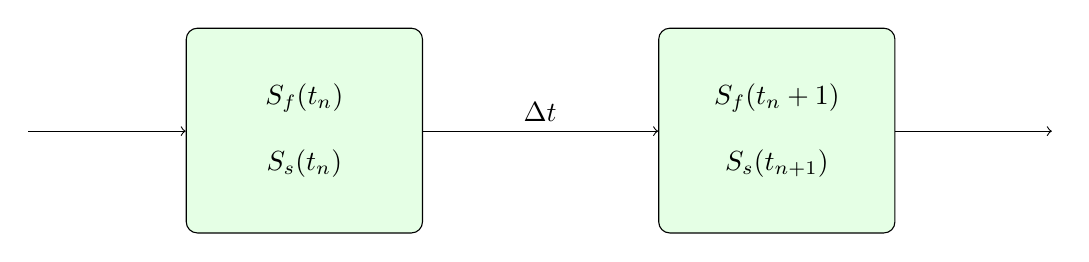
\begin{tikzpicture}[scale=1]


	\tikzstyle{status}=[draw,rectangle,rounded corners,fill=green!10,text centered,inner sep=10pt, anchor=south west, minimum width=3cm,minimum height=2.6cm]
	\draw[->] (0,1.3)-- (2,1.3) node[] {};
	
	\draw[->] (5,1.3)-- (8,1.3) node[midway,above] {$\Delta t$}; % node[midway,below] {step};

	\draw[->] (11,1.3)-- (13,1.3) node[] {};

	\node[status] (t1) at (2,0)  {
		\begin{tabular}{c}
			$S_f(t_n)$ \\
			\\
			$S_s(t_n)$
	\end{tabular}};

	\node[status] at (8,0) {
	\begin{tabular}{c}
		$S_f(t_{n}+1)$ \\
		\\
		$S_s(t_{n+1})$
\end{tabular}};
	
%		\draw (0,1.3) node[below] {$B$} --
%		(3,1.3) node[below] {$C$} --
%		(1.5,4.3) node[above] {$A$} -- cycle;
%		\draw (1.5,4.3) -- (1.5,1.3) node[below] {$D$};
%		\draw (1.5,1.5) -- (1.7,1.5) -- (1.7,1.3);
%		\node[draw,text width=3cm] at (4.5,4) {some text spanning three lines with automatic line breaks};
%		\draw[rounded corners=5pt] (4,0) rectangle ++(2,1);
	\end{tikzpicture}
	\caption{monolithic approach: $S_f$, $S_s$ denote the fluid and the structure solutions}
	\label{fig:monolithic}
\end{figure}


On the other hand, in the \textit{partitioned approach}, the fluid and the solid domains are treated as two distinct computational fields, with their respective meshes, that have to be solved separately (see Figure \ref{fig:partitioned}: how data are passed between solvers is detailed in Section \ref{sec:coupling}). The interface conditions are used explicitly to communicate information between the fluid and structure solutions. This implies that the flow does not change while the solution of the structural equations is calculated and vice versa \cite{degroote2009performance}. The partitioned approach thus requires a third software module (i.e. a coupling algorithm) to incorporate the interaction aspects. It communicates the boundary conditions described in Section \ref{sec:interface}: that is forces or stresses (dynamic data) calculated by the fluid solver at the wet surface are passed to the solid component and displacements or velocities (kinematic data) computed by the solid solver at the interface are sent to the fluid component in return. Finally, fluid and structural solutions together yield the FSI solution.

\begin{figure}[htbp!]
	\centering
	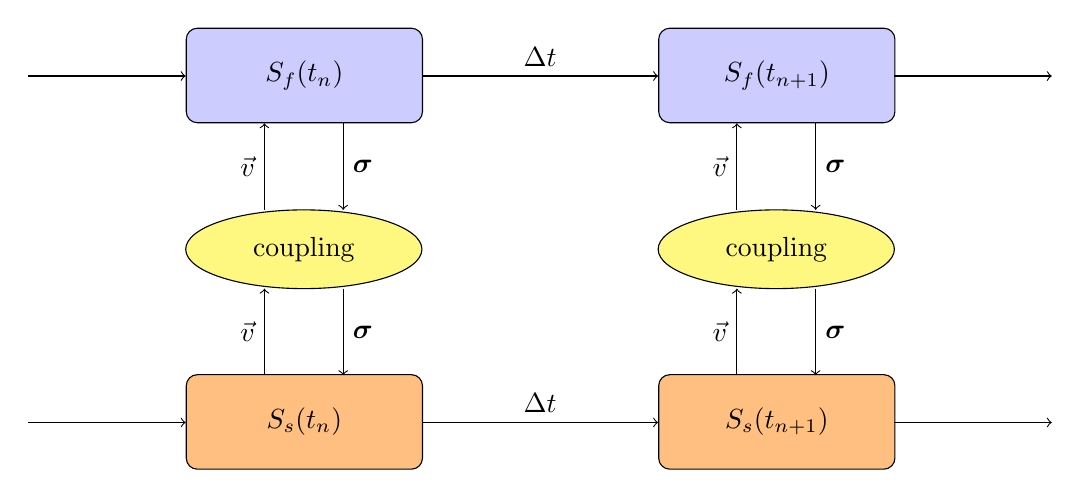
\begin{tikzpicture}[scale=1]

	\tikzstyle{solver}=[draw,rectangle,rounded corners,text centered,inner sep=10pt, anchor=south west, minimum width=3cm,minimum height=1.2cm]
	\tikzstyle{coupling}=[draw, ellipse, fill=yellow!75, minimum width=3cm, minimum height=1.2cm, align=center]

	\node[solver,fill=blue!20] at (2,4.4) {$S_f(t_n)$};
	\node[solver,fill=blue!20] at (8,4.4) {$S_f(t_{n+1})$};
	
	\node[solver,fill=orange!50] at (2,0) {$S_s(t_n)$};
	\node[solver,fill=orange!50] at (8,0) {$S_s(t_{n+1})$};
	
	\draw[->] (0,0.6)-- (2,0.6) node[] {};
	\draw[->] (5,0.6)-- (8,0.6) node[midway,above] {$\Delta t$}; % node[midway,below] {step};
	\draw[->] (11,0.6)-- (13,0.6) node[] {};


	\draw[->] (0,5)-- (2,5) node[] {};
	\draw[->] (5,5)-- (8,5) node[midway,above] {$\Delta t$}; % node[midway,below] {step};
	\draw[->] (11,5)-- (13,5) node[] {};
	
	\node[draw,fill=yellow!50,ellipse,minimum width=3cm, minimum height=1cm] at (3.5,2.8) {coupling};
	\node[draw,fill=yellow!50,ellipse,minimum width=3cm, minimum height=1cm] at (9.5,2.8) {coupling};

	\draw[->] (3,1.2)-- (3,2.3) node[midway,left] {$\vec{v}$};
	\draw[->] (4,2.3)-- (4,1.2) node[midway,right] {$\bm{\sigma}$};

	\draw[->] (3,3.3)-- (3,4.4) node[midway,left] {$\vec{v}$};
	\draw[->] (4,4.4)-- (4,3.3) node[midway,right] {$\bm{\sigma}$};

	\draw[->] (9,1.2)-- (9,2.3) node[midway,left] {$\vec{v}$};
	\draw[->] (10,2.3)-- (10,1.2) node[midway,right] {$\bm{\sigma}$};

	\draw[->] (9,3.3)-- (9,4.4) node[midway,left] {$\vec{v}$};
	\draw[->] (10,4.4)-- (10,3.3) node[midway,right] {$\bm{\sigma}$};
		
	\end{tikzpicture}
	\caption{partitioned approach: $S_f$, $S_s$ denote the fluid and the structure solutions, while $\bm{\sigma}$ and $\vec{v}$ represent coupling data}
	\label{fig:partitioned}
\end{figure}

A big advantage of this approach is that software modularity is preserved: different and efficient solution techniques can be used for the flow equations and structural equations. Provided that they can exchange data, existing solvers for the fluid and solid problem can be reused, ranging from commercial to academic and open-source codes. Those solvers are usually well-validated.
Besides, compared to monolithic procedures, the programming efforts are lower for partitioned approaches, as only the coupling of the existing solvers has to be implemented rather than the solvers themselves.
The challenge of this approach is, however, to define and implement algorithms to achieve accurate and efficient fluid-structure interaction solution with minimal code modification. Particularly, the interface
location that divides the fluid and the structure domains changes in time. The partitioned approach requires that the fluid solver has ALE capabilities, as introduced in Section \ref{subsec:ALE}.
More detailed and practical explanations about the coupling component used in this work are given in Section \ref{sec:precice}. 


\section{Coupling Strategies}
\label{sec:coupling}

Because of the modularity, the partitioned approach has gained much attention in research. The structure sketched in Figure \ref{fig:partitioned} needs to be detailed and specialized in function of the coupling strategies.

In an interface multi-physics coupling like FSI, the boundary surface is in common between the two sides of the simulation. The results make sense and are numerically stable only if the two sides of the interface are in agreement, since the output values of the one simulation become input values for the other (and vice-versa).
The solution strategies can be roughly divided into weakly and strongly coupled approaches. They are often referred to as \textit{explicit} and \textit{implicit} methods in the literature.
When the fluid and solid solutions are computed iteratively until some convergence criteria within the same time step, the scheme is called \textit{implicit coupling}. The faster, simpler but less precise \textit{explicit coupling} consists in executing a fixed number of iterations (typically one per time step) and exchange coupling values without convergence checks. 

\subsection{Explicit coupling schemes}

As in the previous Section, $S_f$ represents the fluid solver, which computes the pressures (named $d_f$ here) at the deformable boundary and $S_s$ is the structure solver, which uses these forces to compute the displacement and velocity of the boundary (named $d_s$). In a \textit{serial-explicit} (or \textit{conventional staggered}) coupling scheme, the solver $S_f$ uses the old time step boundary values $d_s^{(n)}$ to compute the values of $d_f^{(n+1)}$ for the next time step:

\begin{equation}
	d_f^{(n+1)} = S_f\left(d_s^{(n)}\right)
	\label{eq:stag1}
\end{equation}

When the fluid solver completes the time step, data are passed to the structural solver:

\begin{equation}
	d_s^{(n+1)} = S_s\left( d_f^{(n+1)} \right)
	\label{eq:stag2}
\end{equation}

Note that Equation \ref{eq:stag1} uses values computed at $t^n$, while Equation \ref{eq:stag2} uses values computed at $t^{(n+1)}$. The order of execution might be inverted.

In order reduce execution time, the solvers might run in parallel, using data from the same time step (\textit{parallel-explicit coupling}:

\begin{subequations}
\begin{eqnarray}
	d_f^{(n+1)} &=& S_f\left(d_s^{(n)}\right) \\
	d_s^{(n+1)} &=& S_s\left( d_f^{(n)} \right)
	\label{eq:par-exp}
\end{eqnarray} 
\end{subequations}


The two explicit schemes are shown schematically in Figures \ref{fig:serial-explicit} and \ref{fig:parallel-explicit}.

\begin{figure}[htbp!]
	\centering
	\begin{subfigure}{.8\textwidth}
	\centering
	% include first image
		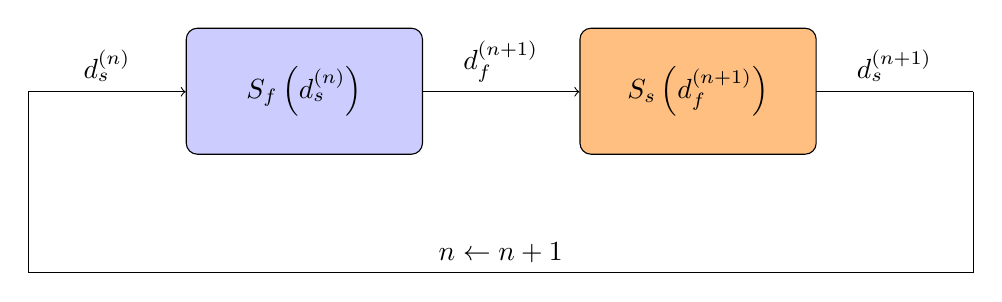
\begin{tikzpicture}[scale=1]
		\tikzstyle{solver}=[draw,rectangle,rounded corners,text centered,inner sep=10pt, anchor=south west, minimum width=3cm,minimum height=1.6cm]
		
		\node[solver,fill=blue!20] at (3,5) {$S_f\left( d_s^{(n)} \right)$};
		\node[solver,fill=orange!50] at (8,5) {$S_s\left(d_f^{(n+1)}\right)$};
		
		\draw[->] (1,5.8)-- (3,5.8) node[midway,above] {$d_s^{(n)}$};
		\draw[->] (6,5.8)-- (8,5.8) node[midway,above] {$d_f^{(n+1)}$};
		\draw[-] (11,5.8)-- (13,5.8) node[midway,above] {$d_s^{(n+1)}$};
		
		\draw[-] (13,5.8)-- (13,3.5);
		\draw[-] (1,5.8)-- (1,3.5);
		
		\draw[-] (1,3.5)-- (13,3.5) node[midway,above] {$n \leftarrow n+1$};
		
		\end{tikzpicture}
		\caption{serial explicit coupling}
		\label{fig:serial-explicit}
	\end{subfigure}
	\newline
	\centering
	\begin{subfigure}{.8\textwidth}
	\centering
	% include second image
		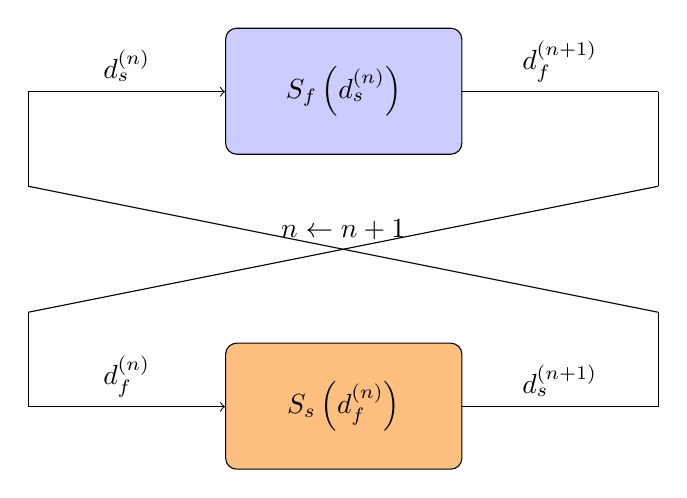
\begin{tikzpicture}[scale=1]
		\tikzstyle{solver}=[draw,rectangle,rounded corners,text centered,inner sep=10pt, anchor=south west, minimum width=3cm,minimum height=1.6cm]

		\node[solver,fill=blue!20] at (2.5,4) {$S_f\left( d_s^{(n)} \right)$};
		\node[solver,fill=orange!50] at (2.5,0) {$S_s\left(d_f^{(n)}\right)$};
		
		\draw[->] (0,4.8)-- (2.5,4.8) node[midway,above] {$d_s^{(n)}$};
		\draw[->] (0,0.8)-- (2.5,0.8) node[midway,above] {$d_f^{(n)}$};

		\draw[-] (5.5,4.8)-- (8,4.8) node[midway,above] {$d_f^{(n+1)}$};
		\draw[-] (5.5,0.8)-- (8,0.8) node[midway,above] {$d_s^{(n+1)}$};
		
		\draw[-] (0,0.8)-- (0,2);
		\draw[-] (8,0.8)-- (8,2);
		
		\draw[-] (0,3.6)-- (0,4.8);
		\draw[-] (8,3.6)-- (8,4.8);
		
		\draw[-] (8,3.6)-- (0,2) node[midway,above] {$n \leftarrow n+1$};
		\draw[-] (0,3.6)-- (8,2);

	
		\end{tikzpicture}
		\caption{parallel explicit coupling}
		\label{fig:parallel-explicit}
	\end{subfigure}
	\caption{Explicit coupling schemes}
\end{figure}

In general, an explicit coupling is not enough to regain the exact (as in the monolithic approach) solution of the problem as the matching coupling conditions between the solvers is not enforced within each time step: no balance between fluid and structural domain with respect to forces and displacements at the interface can be guaranteed (\cite{hou2012numerical}, \cite{degroote2009performance}). Nevertheless, explicit coupling yields good results if the interaction between fluid and solid is weak as in aeroelastic simulations, where in general the simulations show small displacements of the structure within a single time step and the flow field isn't much influenced by the structural displacements (\cite{farhat2006provably}).

\subsection{Implicit coupling schemes}


On the other hand, strongly (implicit) coupling techniques require an iterative method to solve the fixed-point equation that derives from enforcing the agreement of the interface variables.
The coupling conditions at the wet surface are enforced in each time step up to a convergence criterion. If the criterion is not met, another subiteration within the same time instance is computed. Therefore, the solution can approximate the monolithic solution to an arbitrary accuracy.

As in the explicit case, solvers may run in a sequential mode: the coupling is then named \textit{serial} (or staggered) and the solvers wait for each other. 

\begin{subequations}
	\begin{eqnarray}
		d_f^{(n+1),i+1} &=& S_f\left(d_s^{(n+1),i}\right) \\
		d_s^{(n+1),i+1} &=& S_s\left( d_f^{(n+1),i+1} \right)
	\end{eqnarray} 
	\label{eq:ser-imp}
\end{subequations}

Equations \ref{eq:ser-imp} show that, in contrast with explicit coupling, both solvers use interface values at time step $n+1$, but one of them uses data from previous iteration.
If run in parallel mode \cite{mehl2016parallel}, the system becomes:

\begin{subequations}
	\begin{eqnarray}
		d_f^{(n+1),i+1} &=& S_f\left(d_s^{(n+1),i}\right) \\
		d_s^{(n+1),i+1} &=& S_s\left( d_f^{(n+1),i} \right)
	\end{eqnarray} 
	\label{eq:par-imp}
\end{subequations}

At convergence, the following relation holds of serial (or \textit{Gauss-Seidel}) coupling:


\begin{subequations}
	\begin{eqnarray}
		d_s^{(n+1)} &=&  S_s\left(S_f\left(d_s^{(n+1)}\right) \right) \\
		\label{eq:ser-fp-comp}
		d_s^{(n+1)} &=& S_s  \circ S_f \left( d_s^{(n+1)} \right)
	\end{eqnarray} 
	\label{eq:ser-fp}
\end{subequations}


and the following relation holds for parallel (or \textit{Jacobi}) coupling:

\begin{equation}
	\begin{pmatrix}
		d_s^{(n+1)} \\
		d_f^{(n+1)}
	\end{pmatrix} = 
	\begin{pmatrix}
		0 & S_f \\
		S_s & 0
	\end{pmatrix} 
	\begin{pmatrix}
		d_s^{(n+1)} \\
		d_f^{(n+1)}
	\end{pmatrix}
	\label{eq:par-fp}
\end{equation}


Acceleration techniques are necessary to bring fixed point equation \ref{eq:ser-fp-comp} or \ref{eq:par-fp} to convergence. Those techniques are described in Section \ref{sec:strong-coupling}.

The two implicit schemes are shown schematically in Figures \ref{fig:serial-implicit} and \ref{fig:parallel-implicit}: \textit{accel} refers to the post-processing step implemented to speedup convergence. After every non-converged iteration, the latest stored state of the solver (\textit{checkpoint}) is reloaded and coupling iteration \textit{i} for the current time step is incremented. When the solution converges, the time step \textit{n} is incremented.


\begin{figure}[htbp!]
	\centering
	\begin{subfigure}{.8\textwidth}
		\centering
		% include first image
		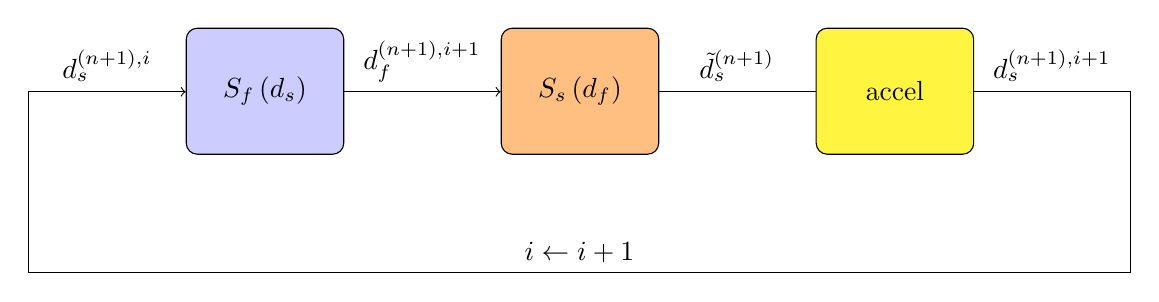
\begin{tikzpicture}[scale=1]
			\tikzstyle{solver}=[draw,rectangle,rounded corners,text centered,inner sep=10pt, anchor=south west, minimum width=2cm,minimum height=1.6cm]
			
			\node[solver,fill=blue!20] at (2,5) {$S_f\left( d_s\right)$};
			\node[solver,fill=orange!50] at (6,5) {$S_s\left(d_f\right)$};
			\node[solver,fill=yellow!75] at (10,5) {accel};
			
			\draw[->] (0,5.8)-- (2,5.8) node[midway,above] {$d_s^{(n+1),i}$};
			\draw[->] (4,5.8)-- (6,5.8) node[midway,above] {$d_f^{(n+1),i+1}$};
			\draw[-] (8,5.8)-- (10,5.8) node[midway,above] {$\tilde{d}_s^{(n+1)}$};
			\draw[-] (12,5.8)-- (14,5.8) node[midway,above] {$d_s^{(n+1),i+1}$};
			
			\draw[-] (14,5.8)-- (14,3.5);
			\draw[-] (0,5.8)-- (0,3.5);
			
			\draw[-] (0,3.5)-- (14,3.5) node[midway,above] {$i \leftarrow i+1$};
			
		\end{tikzpicture}
		\caption{serial implicit coupling}
		\label{fig:serial-implicit}
	\end{subfigure}
	\newline
	\centering
	\begin{subfigure}{.8\textwidth}
		\centering
		% include second image
		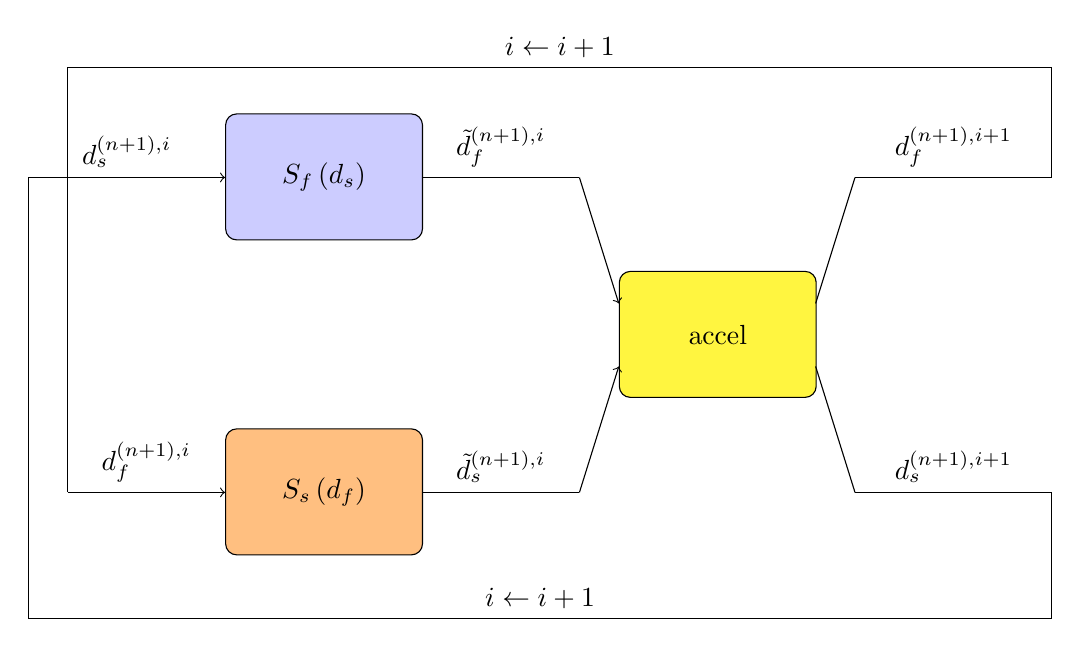
\begin{tikzpicture}[scale=1]
			\tikzstyle{solver}=[draw,rectangle,rounded corners,text centered,inner sep=10pt, anchor=south west, minimum width=2.5cm,minimum height=1.6cm]
			
			\node[solver,fill=blue!20] at (2.5,4) {$S_f\left( d_s \right)$};
			\node[solver,fill=orange!50] at (2.5,0) {$S_s\left(d_f\right)$};
			
			\node[solver,fill=yellow!75] at (7.5,2) {accel};
			
			\draw[->] (0,4.8)-- (2.5,4.8) node[midway,above] {$d_s^{(n+1),i}$};
			\draw[->] (0.5,0.8)-- (2.5,0.8) node[midway,above] {$d_f^{(n+1),i}$};
			
			\draw[-] (5,4.8)-- (7,4.8) node[midway,above] {$\tilde{d}_f^{(n+1),i}$};
			\draw[-] (5,0.8)-- (7,0.8) node[midway,above] {$\tilde{d}_s^{(n+1),i}$};
			
			\draw[->] (7,4.8)-- (7.5,3.2);
			\draw[->] (7,0.8)-- (7.5,2.4);
			
			\draw[-] (10,3.2)-- (10.5,4.8);
			\draw[-] (10,2.4)-- (10.5,0.8);

			\draw[-] (10.5,4.8)-- (13,4.8) node[midway,above] {$d_f^{(n+1),i+1}$};
			\draw[-] (10.5,0.8)-- (13,0.8) node[midway,above] {$d_s^{(n+1),i+1}$};

			\draw[-] (13,4.8)-- (13,6.2);
			\draw[-] (13,0.8)-- (13,-0.8);

			\draw[-] (13,6.2)-- (0.5,6.2) node[midway,above] {$i \leftarrow i+1$};
			\draw[-] (13,-0.8)-- (0,-0.8) node[midway,above] {$i \leftarrow i+1$};
			
			\draw[-] (0,-0.8)-- (0,4.8);
			\draw[-] (0.5,6.2)-- (0.5,0.8);

			%\draw[-] (0,0.8)-- (0,2);
			%\draw[-] (8,0.8)-- (8,2);
			
			%\draw[-] (0,3.6)-- (0,4.8);
			%\draw[-] (8,3.6)-- (8,4.8);
			
			%\draw[-] (8,3.6)-- (0,2) node[midway,above] {$n \rightarrow n+1$};
			%\draw[-] (0,3.6)-- (8,2);
			
			
		\end{tikzpicture}
		\caption{parallel implicit coupling}
		\label{fig:parallel-implicit}
	\end{subfigure}
	\caption{Implicit coupling schemes}
\end{figure}

Implicit methods are generally applicable to any kind of FSI problems, in contrast with explicit methods. When fluid and structure are strongly coupled, explicit coupling can be subject to numerical instabilities, a problem that cannot always be solved by reducing the coupling time step size \cite{van2009added}. These instabilities can be overcome by implicit methods, even if several coupling iterations may be executed every time step, until the values on both sides of the interface converge.


\section{Strong coupling algorithms}
\label{sec:strong-coupling}

As mentioned in the previous chapter, 





\section{Interface Mesh}
\label{sec:interface-mesh}

In this section, FSI methods are classified by means of two different mesh treatment procedures: conforming
or non-conforming techniques. The basic question is, whether fluid and solid mesh need to align
with each other at the FSI interface or not. Unless stated otherwise, the explanations of this section are
taken from [20]. Note that some aspects of conforming mesh methods are already included in the previous
sections without explicitly mentioning so, in order to develop a better understanding of partitioned FSI
simulations.
Conforming mesh methods usually consist of three major subtasks, namely computation in the fluid and
solid domain, as well as interface and mesh movement. They require both fluid and structural meshes
to conform to the wet surface, because the coupling conditions are applied via the interface as physical
boundary conditions for the respective domains. This does not necessarily imply node-to-node matching
of fluid and structure meshes at the interface. This must hold for all time instances, which means that
both fluid and structural grids need to be moved in case deformations of the solid appear. This is a
simple task for the solid mesh, since it is usually expressed in a Lagrangian fashion anyway. However, as
a typical Eulerian fluid mesh would not follow the interface motion, the necessity of the ALE method as
discussed in Section 2.2.3 becomes apparent. Also, mesh smoothing techniques need to be introduced in order to prevent quality losses of the fluid mesh in terms of distorted elements. These irregularities lead
to accuracy loss in simulations. In Figure 3.5, a conforming mesh is shown at two different points in time.
At the first instance (Figure 3.5a) the solid is undeformed and therefore, also the fluid mesh remains in
its initial configuration. In contrast, at the second point in time (Figure 3.5b) the solid is deformed and
the fluid mesh conforms to the displaced wet surface. Consequently, also mesh smoothing is applied.
There is a wide variety of such mesh updating procedures. Some common techniques compute the mesh
movement by considering mesh edges as springs ((torsional) spring analogy), solving the Laplace equation
or solving a pseudo-structural system of equations (see e.g. [18], [43], [20] and their respective references
for further explanations of these techniques). Conforming mesh strategies are widely, but not exclusively
used in partitioned FSI approaches. Furthermore, they typically also utilize the ALE method ([20]).
In contrast, in non-conforming mesh strategies all interface conditions are directly imposed as constraints
on the flow and structural governing equations. Therefore, it is possible to use non-conforming meshes
for fluid and solid domains as they remain geometrically independent from each other. Thus, also mesh
smoothing techniques are obsolete [43]. Figure 3.6 depicts such a situation. By analogy with Figure 3.5,
again the initial configuration (Figure 3.6a) and an instance when the solid is deformed (Figure 3.6b) are
shown. It is clearly visible that the fluid mesh does not conform to the wet surface as all nodes stay at
the same position regardless of the solid deformation.
This approach is mostly used in immersed methods. The considerations in this section are limited to them,
as they are also very common for FSI simulations. Coupling is imposed via additional force-equivalent
terms appearing in the model equations of the fluid, enforcing the kinematic and dynamic conditions.
These FSI forces are computed from the structural model, which is dealt with separately together with
tracking the position of the interface. The forces represent the effects of a boundary or body being
immersed in the fluid domain (leading to immersed boundary and immersed domain methods). A purely
Eulerian mesh can be applied to the whole computational domain for solving the fluid equations, since
the force-equivalent terms are dynamically added in a spatially specific manner to those locations, which
are currently occupied by the structure. After solving the fluid equations, forces exerted on the solid at
the wet surface are computed and used as input for the structural solver, which still employs a Lagrangian
mesh. Subsequently, the deformation of the solid material is calculated and the displacement of the FSI
interface is fed back to the fluid model in form of updated force-equivalent terms ([31], [20], [43]).

\section{Stability: Added Mass Effect}
\label{sec:addedd-mass}

To conclude this chapter about computational aspects of FSI simulations, the AME is briefly described.
Explanations of this effect can be found in a great variety throughout FSI literature, typically explicated
for specific solver strategies or flow regimes (see e.g. [5], [42], [15], [2]). Therefore, in the scope of
this thesis only a short phenomenological introduction to the concept of added mass and numerical
problems arising from it is given. However, this suffices to focus on both weakly and strongly coupled partitioned approaches, which are practically relevant in this thesis. The AME is inherent to partitioned
FSI approaches as the single-physics fields are not continuously coupled but interaction only occurs at a
finite number of discrete time instances, when coupling quantities are exchanged.
As already mentioned in Section 2.3.3, there can be no gaps between structure and fluid. Also their
respective particles cannot occupy the same spatial locations simultaneously. Thus, if the solid is moved,
also fluid particles move. Changing the state of motion of the structural component consequently requires
taking into account inertial effects not only of the solid itself, but also of the surrounding fluid, which
artificially rests for the span of a single structure solver time step. In more descriptive words: Moving the
solid also implies moving fluid particles close to the solid. Therefore, the structure behaves more inert
due to artificially added mass ([42], [2]). Since inertia is dependent on mass and therefore density, the
% AME is also. More precisely, it is dependent on the ratio (MA) of structural (S) und fluid density (F )
([42], [5]):
%MA = S F : (3.1)
This ratio is often used to describe how strong the interaction between solid and fluid is. For cases, in
%which the solid density is much higher than the fluid density (MA  1), this effect does not dominantly
influence the FSI problem (weak interaction). But as fluid and structure densities approach each other
%(MA  1) or the fluid becomes even denser than the solid (MA < 1), its consideration is crucial (strong
interaction) and imposes stability limits on partitioned solution techniques ([5], [42], [2]). Note that the
AME is not only governed by the density ratio of Equation 3.1 but also by geometric properties of the
problem, the stiffness of the solid ([5]) and the speed of sound in the flow domain ([42]). Nonetheless,
for the sake of simplicity and intuitiveness, explanations in this thesis are mostly limited to the density
ratio.
In general, the AME is of bigger concern for incompressible flows than for compressible regimes. From
a physical point of view, deformations of the structural domain can be interpreted as perturbations for
the flow field. In compressible flows the speed of sound (speed at which perturbations propagate through
the flow) is finitely large. Thus, the influence of a geometrical change of the fluid domain caused by
deformations of the solid is locally limited during a certain period of time. In contrast, in incompressible
flows the speed of sound is infinitely large, hence all perturbations propagate through the flow without
time delay. Therefore, regardless of how much time has passed since a perturbation, the whole flow field
is directly affected ([42], [5]).
In the following it is assumed that a weakly coupled algorithm allows computation of the fluid and solid
solution only once per time step. In addition, coupling data is also exchanged once per time instance. In
contrast, a strongly coupled solver does the same at least twice per time increment (for a reminder see
Section 3.2 and compare Figure 3.4). As can be shown, in the compressible case a more dominant AME
can be compensated for by reducing the time step size of strongly coupled, partitioned solution algorithms.
This however, does not hold for the incompressible regime, where even in the limit of vanishing time step
size strongly coupled, partitioned algorithms might fail ([42]). These observations are consistent with the
above mentioned physical explanation.
First of all, considering compressible flows, indeed, the lack of repeated subiterations in weakly coupled
partitioned techniques leads to a strict limit for the density ratio (of Equation 3.1) due to the fact that
the interface conditions are not enforced and energy balance at the wet surface is generally not given.
If that limit is exceeded the algorithm fails due to instability ([2]). Likewise, in such a case a strongly
coupled partitioned algorithm converges slowly, resulting in possibly many necessary subiterations, which
is computationally costly. Yet it does not become unstable, given that the time step size is chosen sufficiently
small. Reducing the time step size to an arbitrarily small extent cannot stabilize a weakly coupled
approach if the stability criterion on the density ratio is not met ([15]). Conversely, the convergence
rate of strongly coupled algorithms increases by the same factor, by which the time step size decreases,
meaning that in the limit of vanishing time step size the monolithic solution is obtained ([5], [42]).
In the incompressible case however, a strict stability limit exists for both weakly and strongly coupled
algorithms. It is independent of the size of time increments1. Furthermore, in order for an implicit
method to achieve the monolithic solution (assuming its convergence is given, i.e. the before mentioned
stability limit is not exceeded) the number of subiterations must be increased as time step size decreases
([15], [42]).
\chapter{Software Packages used in this work}
\label{cha:software}

This chapter illustrates the main software tools used in this work. First, the coupling library \textit{preCICE} is introduced in Section \ref{sec:precice}. Then, the multibody dynamics solver \textit{MBDyn} being connected to preCICE is shortly presented in Section \ref{sec:mbdyn}.


\section{preCICE}
\label{sec:precice}

The main information concerning preCICE is taken from the official documentation: that is \cite{gatzhammer2014efficient} and  \cite{bungartz2016precice}. The preCICE website is also a source of documentation\footnote{\href{http://www.precice.org}{www.precice.org}}.

The open-source\footnote{The code can be accessed via Github: \href{https://github.com/precice/precice}{github.com/precice/precice}} software library preCICE provides the components to connect traditional single-physics solvers and create a partitioned multi-physics simulation (e.g. fluid-structure interaction, conjugated heat transfer, solid-solid interaction, etc.).
It aims at coupling existing solvers in a partitioned black-box manner (see Section \ref{sec:coupling}):  only minimal information abut the solver is available and connection involves just interface nodes. 
In order to be flexible and easily implemented, the impact on the solvers should be as minimal as possible: for this reason, preCICE offers a high level ~\ac{API} (Section \ref{sec:pc-api}) different languages, such as C/C++, Fortran and Python.
The ability to switch among different solvers is advantageous as it provides a lot of flexibility in developing and testing new coupled components.

In a nutshell, preCICE simply affects the input and observes the output of the solvers (called \textit{participants}). The required data and control elements are accessed using an \textit{adapter}, i.e. a "glue code" that is attached to the corresponding solver and communicates the information with the library.

preCICE performs all the actions required to perform a coupled simulation: implements the coupling strategy and convergence criteria (Section \ref{sec:pc-coupling}), the communication
between the participants (Section \ref{sec:pc-comm}), the mapping of data between meshes (Section \ref{sec:pc-map}). preCICE is configured by means of an ~\ac{XML} file (Section \ref{sec:pc-config}).



\subsection{Implemented coupling strategies}
\label{sec:pc-coupling}

The \textit{partitioned approach} (Section \ref{sec:coupling}) is obviously the coupling strategy adopted by preCICE. It allows both \textit{explicit} (Section \ref{subsec:explicit}) and \textit{implicit} coupling (Section \ref{subsec:implicit}). The possible variants are four:

\begin{itemize}
	\item \texttt{serial-explicit}: a serial, weakly coupled algorithm (Figure \ref{fig:serial-explicit}). The first solver uses the second solver solution at the last time step to compute its current solution. In contrast, the second solver needs the current first solution to compute its solution at the same time instance. The order of execution is user defined.
	\item \texttt{parallel-explicit}: both solvers advance in parallel (Figure \ref{fig:parallel-explicit}) and exchange data at the end of each time step, resulting in a less stable procedure. The bottleneck of this procedure is related to the most time consuming solver.
	\item \texttt{serial-implicit}: a serial strongly coupled algorithm (Figure \ref{fig:serial-implicit}). The user can define the order of execution, the coupling algorithm (basically all the algorithms described in Section \ref{sec:strong-coupling}) and its parameters in a section of the configuration file named \texttt{acceleration}.
	\item \texttt{parallel-implicit}: again both solvers execute in parallel (Figure \ref{fig:parallel-implicit}). An implicit scheme modifies the result of the fixed-point iteration on both data \cite{mehl2016parallel}. 
\end{itemize}



\subsection{Communication strategies}
\label{sec:pc-comm}

All the participants need to communicate with each other, in order to share coupling data.
Each solver might be executed in multiple processes or on different nodes of a cluster (\textit{intrafield parallelism}).
This form of parallelization requires efficient forms of communication between the solver in order to avoid that data transfer becomes a bottleneck during a simulation.

preCICE implements a fully parallel process-to-process communication approach \cite{Shukaev2015} using:

\begin{itemize}
	\item \textit{~\ac{MPI}}: available on 	most scientific computers, it may be necessary to adapt/change the MPI versions of the respective single-physics solvers or of preCICE.
	\item \textit{~\ac{TCP/IP}}: popular means of network communication and free of incompatibilities between versions.
\end{itemize}

As to performances, MPI is the best technique especially when a high numbers of nodes is present. Anyway, socket communication is quite as fast, such that
both techniques are very well-suited for larger-scale simulations \cite{gatzhammer2014efficient}.

In each solver, executed in parallel, one "master" process is defined to manage the progress of the simulation. No central node is required. The participating
processes use asynchronous point-to-point (M:N) communication. The channels are static and defined in the beginning of the simulation. This sets a limit in using preCICE with dynamically adaptive meshes or immersed boundaries.

\subsection{Data mapping}
\label{sec:pc-map}

Even if volume coupling is possible, preCICE is mainly designed to couple simulations that share a common surface boundary (namely \textit{conforming meshes}, in the terminology used in Section \ref{sec:conforming-mesh}). The meshes don't need to be node-to-node coincident, so it is necessary to map variables at the interface, preserving the geometry (i.e. no gaps or superpositions at the interface) and the mass and energy balances. 

The user defines which data are shared by each \textit{participant} (i.e. solver) and the way data is shared in the configuration section named \texttt{mapping}. As described in Section \ref{sec:data-mapping}, two kinds of mapping are available:

\begin{itemize}
	\item \texttt{consistent}: the value of a node at the one grid is the same as the value of the corresponding node (or nodes) at the other grid. In general the number of fluid nodes is at least the same or, more often, exceeds the nodes of the structure, so a single structural node is associated to several fluid nodes. The mapping of displacements is consistent: in the simplest case, all fluid nodes experience the same displacement of a single solid node, otherwise an interpolation is performed (see Figure \ref{fig:consistent}).
	\item \texttt{conservative}: in the same conditions as before, forces are mapped from multiple fluid nodes to a single solid node in an additive manner (see Figure \ref{fig:conservative}).
\end{itemize} 

Along with the mapping strategy, a method must be defined (see Section \ref{sec:data-mapping}): \texttt{nearest-neighbor}, \texttt{nearest-projection}, \texttt{rbf}. For the latest method, preCICE implements a wide variety of basis functions, with Gaussian and thin plate splines being the most widely used.

 

\subsection{Configuration}
\label{sec:pc-config}

In order to run a multi-physics simulation with preCICE, all the participating, \textit{adapted} solvers have to be started (the order is irrelevant).
Some configuration files are needed:

\begin{itemize}
	\item each adapter in general needs its own configuration file. It normally contains information about the boundaries (wet-surface) used for the coupling, names of exchanged data, mesh and the name of the common preCICE configuration file, plus other parameters, specific to the adapter. The one for the MBDyn adapter will be described in more detail in Chapter \ref{cha:adapter} and in Appendix \ref{app:mbd-config-file}.
	\item preCICE configuration file: This is an XML file and each participant points at it. It defines all the information relevant to the simulation:
	\begin{itemize}
		\item type and name of exchanged data and meshes over which those data are passed
		\item which solvers participate in the simulation, which data produce or consume, and how the mapping is performed
		\item how solvers communicate among each other
		\item coupling scheme and all the necessary information 
	\end{itemize}
	
	The structure of a preCICE configuration file is illustrated in Appendix \ref{app:pc-config-file}.
		
\end{itemize}


\subsection{Application Program Interface}
\label{sec:pc-api}

A solver, in order to be coupled to preCICE, must either provide a way to access its core functions (e.g. initialize, set input data, read output, advance...) from outside the code (via API, socket, etc...) or it has to be slightly modified in order to perform all the operations required by the preCICE library.

The result is an \textit{adapter}, which can be the modified and recompiled original solver, or a standalone piece of code that communicates with the original unmodified solver on one side and with the preCICE library on the other. The adapter groups together all the calls to the preCICE methods from its API (a list of the API calls, taken from the official documentation, can be found in Appendix \ref{sec:api-code}).

While preCICE is written in C++, there exist APIs also for other languages, so that the adapter can be written also in C, Fortran or Python.

A coupling consists of a configuration and an initialization phase, multiple coupling advancements and a finalization phase: the general structure of an adapter can be found in \ref{sec:adapter-code}.


\subsection{Official Adapters}
\label{sec:pc-adapters}


This work introduces an adapter to preCICE for MBDyn. It is based on previous MBDyn adapters and on the examples given on the preCICE website\footnote{\href{https://github.com/precice/precice/wiki/Adapter-Example}{github.com/precice/precice/wiki/Adapter-Example}}.
Official adapters are currently available for several free solvers, e.g. CalculiX, Code-Aster and SU2. Also some closed-source software packages are supported. A (maybe outdated) list of official adapters can be found in \cite{uekermann2017official}, while the current status of coupled codes can be found at the following link: \href{https://www.precice.org/codes/}{preCICE adapters}.


\section{MBDyn}
\label{sec:mbdyn}


MBDyn is free and open-source\footnote{the software is available through a public git repository \href{https://gitlab.polimi.it/Pub/mbdyn}{gitlab.polimi.it/Pub/mbdyn}} general purpose Multibody Dynamics analysis software developed at the \textit{Dipartimento di Scienze e Tecnologie Aerospaziali}  of the University Politecnico di Milano.

Most of the information concerning MBDyn is taken from the official documentation given in the software website\footnote{MBDyn website: \href{https://www.mbdyn.org/}{mbdyn.org}} and form the input manual\footnote{a copy can be found at the following link [\href{https://www.mbdyn.org/userfiles/documents/mbdyn-input-1.7.3.pdf}{input manual}] or in the code repository}.

MBDyn allows to build a simulate multibody system, which\footnote{see Wikipedia entry: \href{https://en.wikipedia.org/wiki/Multibody_system}{Multibody system}} is the study of the dynamic behavior of interconnected rigid or flexible bodies, each of which may undergo large translational and rotational displacements.

MBDyn can simulate linear and non-linear dynamic or rigid and flexible bodies (including geometrically exact and composite-ready beam and shell finite elements, component mode synthesis elements, lumped elements) subjected to kinematic constraints, external forces and control subsystems\cite{masarati2014efficient}. 
MBDyn has been developed to serve as an analysis tool for rotorcraft research and cab simulate essential fixed-wing and rotorcraft aerodynamics.

As explained more in detail later, MBDyn is open to be connected to other software components to perform multiphysics simulations. In particular, it is possible to pass externally computed forces  and to steer the multibody simulation from an external API: this feature has been particularly useful in building and \textit{adapter} to couple MBDyn with the library preCICE (see Chapter \ref{cha:adapter}).

In this section we give a short introduction to some of the relevant features of MBDyn, starting form basic information on the input file syntax (Section \ref{sec:mbd-syntax}), and the output files (Section \ref{sec:mbd-output}). Then some of the elements relevant for the description of the models used in the this work are presented: nodes (Section \ref{sec:mbd-node}), beam elements (Section \ref{sec:mbd-beam}), bodies (Section \ref{sec:mbd-body}) and forces (Section \ref{sec:mbd-forces}). 


\subsection{Basic syntax}
\label{sec:mbd-syntax}

MBDyn is a command line tool and can be generally started from a terminal passing an input file containing all the information required to perform a simulation. 

The input files is structured in blocks and each block has a syntax described in Backus Naur form in the input manual.

\lstset{language=mbdyn}
\begin{lstlisting}[caption=MBDyn input file structure,label=lst:mbd-struct]
begin : data ;
    # select a problem
    problem : initial value ;
end : data ;

begin : initial value ;
    # problem-specific data
end : initial value ;

begin : control data ;
    # model control data
end : control data ;

begin : nodes ;
    # nodes data
end : nodes ;

begin : elements ;
    # elements data
end : elements ;
\end{lstlisting}

As illustrated in listing \ref{lst:mbd-struct}, statements are logically divided in blocks. Each block is opened by a \texttt{begin} statement and it is closed by an \texttt{end} statement.

The sequence of relevant valid blocks is:

\begin{itemize}
    \item \texttt{data}: defines the kind of problem to be solved by the analysis. The most significant one is \texttt{initial value} and is already defined in the example. 
    \item type of problem:  block takes the name of the problem defined in the data block (\texttt{initial value} in this case) and contains all the information required by the integration method to perform the desired simulation (e.g. simulation type, time step, number of iterations, tolerance ...).
    \item \texttt{control data}: mostly contains information about the problem that is required to ensure that a consistent model will be generated (i.e. the number of nodes, elements, forces...).
    \item \texttt{nodes}: The nodes block contains all the nodes required by the simulation. They are are defined as the entities that make degrees of freedom available to the simulation, so they must exist before any element is generated.
    \item \texttt{elements}: contains all the elements. They are defined as the entities that generate equations using the degrees of freedom provided by the nodes.
\end{itemize}

We focus now on the main entities of a MBDyn simulation, namely nodes and elements. A detailed example of the input file used in most simulations in this work can be found in Appendix \ref{sec:mbdyn-input-file}.


\subsection{Nodes}
\label{sec:mbd-node}

Nodes are the basic blocks of a model: they instantiate kinematic degrees of freedom and the corresponding equilibrium equations. There can be different type of nodes in MBDyn, we focus here on \texttt{structural nodes}.

Structural nodes can have 3 degrees of freedom, thus describe the kinematics of point mass motion in space  (position) or 6 DoFs (position and orientation), and thus describe the kinematics of rigid-body motion in space.

Each node has a unique label and can be specified in different ways:

\begin{itemize}
	\item \texttt{static}: this keyword instantiates only equilibrium equations (force for 3 DoF nodes or force and moment for 6 DoF nodes)
	\item \texttt{dynamic}: this also instantiates momentum (3 and 6 DoFs) and momenta moment (6 DoFs)
\end{itemize}

Also \texttt{modal} and \texttt{dummy} nodes exist, but are beyond the scope of this work.

Nodes are the starting point to define the elements of a simulation.


\subsection{Elements}
\label{sec:mbd-elem}

Elements constitute the components of the multibody model. Each has a unique numerical label and is connected to one or more nodes. They write contributions to nodes equations and represent \textit{connectivity} and \textit{constitutive properties}.

%Elements that require both displacement and orientation can only be connected to 6 DoFS nodes.

There exist many types of elements in MBDyn, we focus here on the ones used in the FSI simulation: beams, bodies, joints and forces.



\subsection{Beam elements}
\label{sec:mbd-beam}

As briefly introduced in Section \ref{sec:beam}, when simulations involve slender bodies, it is particularly interesting to use a 1D finite element model together with a form of mapping between the interface (wet surface) and the model to exchange kinematics and dynamics information. This can be performed in MBDyn using \texttt{beam} elements (described in this section) and the \texttt{external structural mapping} element (described in Section \ref{sec:mbd-forces}).

MBDyn models slender deformable components by means of finite volume \texttt{beam} elements with a high level of flexibility.

The beam element is defined by its nodes and a reference line; although 2 and 3 nodes beam elements are implemented, only \texttt{beam3} are considered here (Figure \ref{fig:mbdyn-beam-model}). Each node of the beam is related to a \texttt{structural node} (node 1 to 3 in Figure \ref{fig:mbdyn-beam-model}) by an offset ($o_1$ to $o_3$) and a relative orientation.

\begin{figure}[htbp!]
	\centering
	\includegraphics[width=0.8\textwidth]{images/beam_model}
	\caption{MBDyn beam model, taken from the input manual}
	\label{fig:mbdyn-beam-model}
\end{figure}


The Finite Volume approach described \cite{ghiringhelli2000multibody} is used to model the beam element. It computes the internal forces as functions of the reference line strain and as functions of the  orientation at the \textit{evaluation points} (i.e. integration points, point I and II in Figure \ref{fig:mbdyn-beam-model}) that are between nodes 1 and 2, and between nodes 2 and 3 (at $\xi =-1/\sqrt{3}$ and $\xi = 1/\sqrt{3}$ of a non-dimensional abscissa $-1\leq \xi \leq 1$ ranging from node 1 to node 3).


A 6D constitutive law is defined at each evaluation point: it relates the strains and the curvatures of the beam (and their time derivatives) to the internal forces and moments at the evaluation points in the form:

\begin{equation}
	\begin{Bmatrix}
		F_x \\ F_y \\ F_z \\ M_x \\ M_y \\ M_z
	\end{Bmatrix} = f
	\begin{pmatrix}
		\begin{Bmatrix}
			\epsilon_x \\ \gamma_y \\ \gamma_z \\ \kappa_x \\ \kappa_y \\ \kappa_z
		\end{Bmatrix} , 
		\begin{Bmatrix}
			\dot{\epsilon_x} \\ \dot{\gamma_y} \\ \dot{\gamma_z} \\ \dot{\kappa_x} \\ \dot{\kappa_y} \\ \dot{\kappa_z}
		\end{Bmatrix}
	\end{pmatrix}
\end{equation}


Using the convention of \textit{x-axis} as beam axis we have:

\begin{itemize}
	\item $F_x$: axial force component,
	\item $F_y$ and $F_z$: shear force components,
	\item $M_x$: torsional moment component,
	\item $M_y$ and $M_z$: bending moment components,
	\item $\epsilon_x$: axial strain component,
	\item $\gamma_y$ and $\gamma_z$: shear strain components,
	\item $\kappa_x$: torsional curvature component,
	\item $\kappa_y$ and $\kappa_z$: bending curvature components,
	\item $f$: constitutive law.
\end{itemize}


\subsubsection{Beam section Constitutive Law}

In dynamic simulations, linear elastic or viscoelastic laws are generally used, even though nonlinear laws can be used.  Focusing on linear laws, MBDyn allows the user to define every constitutive laws, going from an isotropic beam section to a fully anisotropic one: in fact the entire $6 \times 6$ constitutive matrix can be provided. It is up to the user to define a valid law as the matrix must satisfy some constraints, e.g. it must be symmetric.

In the context of FSI simulations, this feature allows the user to define a section constitutive law that is independent from the shape of the beam itself. Thus the aerodynamic aspects and the structural aspects are handled by two distinct elements of the model: i.e. the interface mesh defines the aerodynamic forces and the beam constitutive law defines the structural properties.   

Some studies about the definition of general beam section constitutive properties (\textit{composite beam section characterization}) are available in the literature: an early work can be found in \cite{giavotto1983anisotropic}, a review in \cite{hodges1990review} or an application to wind turbine blades in \cite{kim2013development}.


\subsection{Bodies}
\label{sec:mbd-body}

The \texttt{body} element describes a lumped rigid body when connected to a regular, 6 DoF structural node, or a point mass when connected to a rotationless, 3 DoF structural node. It can be used in connection with a structural element to give inertial properties: for example, in a \texttt{beam} element (see Section \ref{sec:mbd-beam}), 2 bodies are added to the evaluation points of the beam to account for lumped inertia of each portion in which the beam is divided. 


\subsection{Joints}
\label{sec:mbd-joint}

\texttt{structural} nodes can be constrained by means of \texttt{joint} elements. Many different joints are available. In the FSI model the following types of joints are used:

\begin{itemize}
	\item \texttt{clamp}: grounds all 6 DoFs of a node in an arbitrary position and orientation
	\item \texttt{total joint}: allows to arbitrarily constrain specific components of the relative position and orientation of two nodes\cite{masarati2013formulation}
\end{itemize}


\subsection{Forces}
\label{sec:mbd-forces}

The \texttt{force} element is a general means to introduce a right-hand side to the equations. Structural forces are specific to structural
nodes and  have three components that may depend on arbitrary parameters and a location in space.

MBDyn allows to communicate with an external software that computes forces based on information on the kinematics of the model. This feature is at the basis of the development of the \textit{adapter}. The following elements can be used.


\subsubsection{External Structural}

The \texttt{External Structural} element allows to communicate with an external software that computes forces applied to a pool of \texttt{nodes} and may depend on the kinematics of those nodes. In this case forces are applied directly to the nodes. In a FSI model, this would require that each interface mesh node has a correspondent MBDyn structural node. 

\subsubsection{External structural mapping}

This element is similar to the previous one, but the nodes where forces are applied and the kinematics is computed depend on structural nodes through a linear mapping. This element has been used in building the adapter. In order to use the \texttt{external structural mapping} elements, the following steps have to be performed:

\begin{enumerate}
	\item a set of points is defined for each \texttt{structural node} according to a specified offset. Those points are used to compute the kinematics of the interface points, originating from the rigid-body motion of the structural nodes
	\item before the simulation, a linear mapping matrix $H$ is generated starting from the position of the above points and the interface mesh points (this is performed by means of an \texttt{Octave} script which is part of MBDyn). The matrix is stored in sparse form
	\item the mapping matrix is used during simulation to map forces and kinematics between the interface nodes and the structural nodes
\end{enumerate}

The constant matrix mapping allows to compute the position and the velocity of the \textit{interface} points as function of the points rigidly offset from structural nodes:

\begin{subequations}
	\begin{eqnarray}
		x_{interf} &=& H x_{mbdyn} \\
		\dot{x}_{interf} &=& H \dot{x}_{mbdyn} 
	\end{eqnarray}
\end{subequations}

The same matrix is used to map back the forces onto structural nodes based on the preservation of the work done in the two domains:

\begin{equation}
	\delta x_{mbdyn}^T \cdot f_{mbdyn} =  \delta x_{interf}^T \cdot f_{interf} = \delta x_{mbdyn}^T \cdot H^T \cdot f_{interf} 
\end{equation}

which implies

\begin{equation}
	f_{mbdyn} = H^T f_{interf}
\end{equation}

When performing an FSI simulation with strong coupling (see Section \ref{sec:strong-coupling}), MBDyn may need to compute multiple iterations of the same time step in order to reach global convergence. This is performed by using the keyword \texttt{tight} in the coupling of the \texttt{external structural mapping}. The computation and the communication pattern is the following:

\begin{enumerate}
	\item MBDyn sends the predicted kinematics for time step $k$
	\item MBDyn receives a set of forces sent by the external peer; those forces are computed based on the kinematics at iteration $j$
	\item MBDyn continues iterating until convergence using the last set of forces until, while reading the forces, it is informed that the external peer converged. this implies that MBDyn solves the kinematics for time step $k$ at iteration $j$ using the forces evaluated by the external solver for iteration $j-1$ 
\end{enumerate}

The communication with the external software, in our case the adapter itself, is performed by means of a local unix socket.


\subsection{Simulation output}
\label{sec:mbd-output}

There are a bunch of output files regarding a simulation performed with MBDyn. the name of those files is specified with the option \texttt{-o} (otherwise the name is the same as the input file) and the extensions are:

\begin{itemize}
    \item \texttt{.out}: for miscellaneous output
    \item \texttt{.mov}: for kinematic output of the nodes
    \item \texttt{.ine}: for the dynamic output of the nodes
    \item \texttt{.frc}: for the output of force elements
    \item \texttt{.act}: for the output of beam elements
    \item \texttt{.jnt}: for the output of joint elements
\end{itemize}

The \texttt{.out} file contains information regarding the simulation iterations residuals while other files are described in more detail in Appendix \ref{sec:mbdyn-output-file}.



%
%output
%
%If we copy the above written code to a file called, say, “rigidbody”, and invoke
%mbdyn -f rigidbody
%after a while we obtain the results of the simulation in a set of files called “rigidbody.<ext>”.
%In this case, the extensions will be:
%• out for miscellaneous output
%• mov for the kinematic output of the node
%• ine for the dynamic output of the node
%• frc for the output of the force
%The first file (out) will be ignored at present. The second file (mov) will contain Nnodes
%by Ntimesteps lines formatted as:
%• the node label
%• the three coordinates of the position of the node
%• the three Euler-like angles that define the orientation of the node (following the
%1, 2, 3 convention)
%• the three components of the velocity of the node
%• the three components of the angular velocity of the node
%all the above mentioned quantities are expressed in the global inertial frame
%




\chapter{MBDyn Adapter and its integration}
\label{cha:adapter}


To prepare an existing simulation code for coupling, preCICE has to be integrated with the solver, using  API described in Section \ref{sec:pc-api} and in Appendix \ref{sec:api-code}. The "glue-code" required for this operation is called \textit{adapter}, as depicted in Figure \ref{fig:adapter-scheme}.


\begin{figure}[htbp!]
	\centering
	\includegraphics[width=0.92\textwidth]{images/adapter_scheme}
	\caption{Coupling CFD to CSM via preCICE.The existing solver code, the adapter and the linked library are highlighted (image taken from \cite{uekermann2017official}).}
	\label{fig:adapter-scheme}
\end{figure}


\section{Design of the adapter structure}


In order to couple MBDyn with preCICE a C++ adapter has been implemented within the scope of this work. The \textit{adapter} needs to be integrated with both the MBDyn solver and the coupling library. The two connections are distinct but strictly interconnected.
The adapter has the advantage of being completely independent from both the preCICE library and MBDyn. The first connection is achieved via the API given by the library \texttt{libprecice.so}, the second connection exploits the API given by MBDyn through its library \texttt{libmbc.so}.


\section{Structure of the code}

The code for the adapter is available through a public git repository\footnote{\href{https://gitlab.com/Ccaccia73/mbdyn-adapter-test/-/tree/develop}{mbdyn-beam-adapter}}. The code is conceptually divided in two classes, as illustrated in Figure \ref{fig:adapter-classdiag}.

The main class is \texttt{MBDynAdapter}, which implements the functions given by the preCICE interface. It has access to the class \texttt{MBDynConnector} which takes care of all the aspects regarding MBDyn. Attributes, methods and operations of each class are briefly described in the following sections.

\begin{figure}[htbp!]
	\centering
	\includegraphics[width=0.8\textwidth]{images/classdiag2}
	\caption{MBDyn adapter class structure}
	\label{fig:adapter-classdiag}
\end{figure}


\subsection{Class MBDynAdapter}
\label{sec:mbdyn-adapter.h}

The file \texttt{MBDynAdapter.h} and its source file \texttt{MBDynAdapter.cpp} implements all the methods required to perform and FSI simulation with MBDyn as the solid solver. The basic steps are:

\begin{enumerate}
	\item prepare the MBDyn solver,
	\item prepare the interface,
	\item provide access to the mesh and initialize the coupling data,
	\item steer the coupled simulation,
	\item finalize the simulation.
\end{enumerate}

\subsubsection{Initialization}

In the initialization phase, the instance of \texttt{MBDynAdapter} gets a \texttt{json} file (see Section \ref{sec:mbdyn-adapter-input}) that contains all the parameters useful for the simulation.
Then it instantiates the \texttt{MBDynConnector} (see Section \ref{sec:mbdyn-connector.h}) which takes care of all the operations concerning MBDyn: in particular starting the simulation the creating an instance of \texttt{MBCNodal} in order to have access to the simulation.

In the next step an instance of \texttt{precice::SolverInterface} is initialized and configured with all the relevant information data:

\begin{itemize}
	\item preCICE configuration file (see Section \ref{sec:pc-config} and Appendix \ref{app:pc-config-file}).
	\item \textit{participant} (i.e. solver) name
	\item information regarding the data to be read and written
\end{itemize} 

The next initialization step concerns the definition of the interface mesh. The data concerning the vertices is stored in the \texttt{MBDynConnector} to be used to plot the output and is passed to the \texttt{SolverInterface} to define the wet surface nodes. The mesh nodes are stored in the same text file that is used by MBDyn to build the \texttt{external structural mapping} information (see Section \ref{sec:mbd-forces}). This means that the MBDyn mapped points coincide with the interface mesh on the structural side (note that it doesn't have to be the same mesh of the fluid side, as preCICE can map non identical meshes, as described in \ref{sec:pc-map}). The suitable size of memory is then initialized to contain the coupling information: mainly \textit{displacements}, to be written on the preCICE interface, and \textit{forces}, to be read from the interface.


\subsubsection{Execution}




\subsubsection{Finalization}

In the finalization phase all the object used during the simulation are closed and memory released.



\subsection{Class MBDynConnector}
\label{sec:mbdyn-connector.h}

- mbdynConnector: connection to MBDyn



\section{Input parameters}
\label{sec:mbdyn-adapter-input}

input: json config file

- simulation parameters

\section{Output results}

output: VTK and resultants





%In order to couple SU2 with preCICE, a C++ adapter class named Precice1 is developed in the scope of
%this work. A header file precice.hpp and a source file precice.cpp are the practical outcome. The Precice
%class encapsulates all coupling related activities and separates them from the original SU2 source code.
%It makes use of the high-level API provided by preCICE. Since the adapter is integrated into the source
%code of SU2, it is completely compiled with it (for a description on how to install SU2 with preCICE,
%see Appendix B). This way, coupling is achieved with minimally invasive code changes in SU2 and an
%adaption of the original code is, thus, possible with only small effort, basically reduced to copy-paste
%tasks. The adapter allows for usage of both explicit and implicit coupling strategies implemented in
%preCICE and fully conforms with intra- and interfield parallelism. Moreover, usage of the adapter is
%assimilated to the regular configuration process of SU2, thus, it is embedded smoothly into the software
%suite. All options concerning the usage of preCICE (e.g. switching it on or off, specifying name and
%location of the preCICE configuration file, etc.) are set via the SU2 configuration file. Consequently, no
%recompilation of SU2 is necessary when the user decides to use/not to use preCICE. In addition, a single
%executable, SU2_CFD, is enough to account for single-physics simulations (without preCICE) as well as
%for FSI computations via preCICE. Figure 5.1 shows a schematic representation of the code coupling
%approach.
%Concerning notation of code shown in this chapter (and in the corresponding referenced sections of the
%appendix), it is important to state that SU2 uses several "containers" for storing information (technically,
%they are multiple pointers). E.g. a "config_container” is an instance of CConfig or a "geometry_container"
%refers to CGeometry. Furthermore, all shown code excerpts are reduced to the necessary information.
%Therefore, not all arguments of functions are stated but only the relevant ones. Also, ellipses (...) are
%used to denote further lines of code, which are not shown for the sake of simplicity.
%This chapter is organized in the following top-down way: Starting from the most user-respective changes
%in SU2, in Section 5.1, the newly added, coupling-related options included in the SU2 configuration
%file are presented and their usage is explained. In addition, necessary code changes are stated. The
%chapter continues with a more technical, detailed description on how the coupling is embedded in SU2,
%as in Section 5.2 adaptions to the main routine of SU2_CFD are described. Mostly, these modifications
%include calling several functions, which are incorporated in the adapter class Precice. However, the tasks
%hidden in these functions are not described until finally, the adapter itself is extensively explained with
%emphasis on both physical and computational details at the end of this chapter in Section 5.3. Referring
%back to Figure 5.1, Sections 5.1 and 5.2 correspond to "code changes" in SU2, while Section 5.3 relates
%to the "Coupling Adapter".
%5.1 Changes Concerning SU2 Configuration
%In order to fully control the usage of preCICE for FSI simulations within SU2, new options in the
%configuration file of SU2 are available (for a recapitulation of this file, see Section 4.2.2). They are listed
%in the following with their default values:
%PRECICE_USAGE = NO, YES (5.1a)
%PRECICE_CONFIG_FILENAME = precice.xml (5.1b)
%PRECICE_VERBOSITYLEVEL_HIGH = NO, YES (5.1c)
%PRECICE_WETSURFACE_MARKER_NAME = wetSurface (5.1d)
%Most obvious, PRECICE_USAGE is a flag used for determining whether a simulation should be run
%with or without preCICE. Modifying the remaining three options is only reasonable if it is set to YES.
%PRECICE_CONFIG_FILENAME specifies the name of the configuration file of preCICE. Also, its path
%relative to the location of the SU2 configuration file must be specified. In order to allow users to have more
%insight into the sequence of activities within the coupling adapter, the level of verbosity of the adapter can
%be chosen. If PRECICE_VERBOSITYLEVEL_HIGH is set to YES, several checkpointing information
%of the adapter is output to the console. Yet, too much console output can slow down simulations. Since
%this information is typically not relevant when running an FSI simulation productively, the verbosity level
%is chosen to be low by default. This feature of the coupling adapter is mainly included for tracing back
%runtime errors. Eventually, as explained in Section 4.2.2, physical boundaries are treated as markers in
%SU2. Each boundary has a unique identifying name, which is specified in the SU2 mesh file. The boundary
%marker name corresponding to the FSI interface of the fluid mesh must be passed to the coupling adapter,
%which is done via the option PRECICE_WETSURFACE_MARKER_NAME. A description on how to
%adapt SU2 in order to use the new configuration options is given in Listings A.1, A.2 and A.3, Appendix
%A to a detailed level.
%The dynamic mesh capabilities of SU2 must be enabled, in order to use the implemented ALE formulation
%of the flow solver. This is done via:
%GRID_MOVEMENT = YES (5.2)
%Still, a specific kind of grid movement needs to be chosen. Intrinsically available are e.g. specifications
%for rigid motions or rotations of the mesh. Here, a new option is available, which is mandatory if SU2 is
%used for FSI simulations via preCICE:
%GRID_MOVEMENT_KIND = PRECICE_MOVEMENT (5.3)
%A manual on how to add this new grid movement option to the configuration procedure of SU2 is given
%in Listing A.4, Appendix A.
%Yet, the implementation of PRECICE_MOVEMENT is missing. It defines the steps of which the mesh
%movement procedure consists. After displacements of the nodes at the wet surface are transferred to
%SU2 via preCICE, the mesh needs to be deformed and smoothed (for a reminder, see Sections 2.2.3 and
%3.3). Despite the sole mesh deformation, also grid velocities must be calculated in order to be able to
%use the ALE method of SU2. Finally, for cases in which the SU2 multigrid capabilities are enabled,
%displacements and velocities of the mesh nodes need to be mapped to all grid levels. Intrinsic SU2
%mesh movement procedures cannot be reused as either they do not include the three necessary steps
%stated above (mesh deformation, grid velocity computation, forwarding information to multigrid levels)
%or they involve further computations, which are not necessary for FSI simulations and therefore, represent
%unnecessary computation overhead. The code defining the steps of PRECICE_MOVEMENT is given in
%Listing A.5, Appendix A.
%
%5.2 Adaption of SU2 Main Routine
%After modifying files related to the configuration procedure of SU2 in the previous section, it remains to
%adapt the SU2_CFD module in SU2_CFD.cpp, which relates to the solver run procedure itself. The goal
%is to add as little code as possible in the main solver routine of SU2 such that the coupling adapter can
%be used. Detailed, corresponding code excerpts are stated in Appendix A.
%One core criterion for integrating the adapter into SU2 is that the solver executable should be able
%to run both single- and multiphysics simulations without recompilation. Only a single adapter-related
%variable needs to be initialized in the main routine of SU2 regardless of whether preCICE is used for a
%simulation or not. The variable (called precice_usage) is a boolean flag corresponding to the newly added
%PRECICE_USAGE option of the SU2 configuration file. This flag is the basis for conditionally triggering
%all coupling activities. If it is set to false, no more coupling variables are initialized in SU2_CFD and
%the single-physics solver runs according to the regular scheme previously shown in Algorithm 2, Section
%4.2.2. The (only three) additional variables needed for coupling include an instance of the adapter class
%Precice and two time-stepping variables (namely max_precice_dt and dt).
%preCICE needs to be able to shut down SU2, in case the FSI simulation should be ended. Therefore, an
%adaption of the main solver while-loop is necessary. In case a simulation runs without preCICE, the usual
%condition of the while-loop is used, which checks that the number of solver iterations is smaller than a
%specified maximum. However, if a coupled FSI simulation is executed, the adapter additionally evaluates
%if preCICE signalizes a solver shut down.
%Assuming that the solver loop is executed, a checkpointing procedure for implicit coupling strategies of
%preCICE starts. For strongly coupled algorithms, preCICE tries to find the fixed-point of the coupling
%equation system (as explained in Section 4.1.1). If the solution of a subiteration does not satisfy the pre-
%CICE convergence criteria, resetting the fluid solver to the start of the time step is necessary. Therefore,
%at the beginning of each solver iteration in SU2, the current solver state is saved such that reloading it
%becomes possible. However, this is only done in the first subiteration of a new time step.
%As mentioned in Section 4.1, preCICE might need to enforce time step sizes for the single-physics solvers.
%To allow for the same in SU2, the minimally allowed time step size for an iteration needs to be determined
%before the solution procedure starts. Here, the variables dt and max_precice_dt come into play. While
%the former stores the current time increment of SU2, the latter is the maximum prescribed by preCICE.
%After SU2 is done with executing a single solver iteration, preCICE is informed that a new flow solution
%is available. Therefore, the coupling tool might advance in time. This triggers preCICE to manage the
%data exchange between SU2 and other coupled solvers, as well as to execute the coupling algorithm. In
%case of an implicit procedure, convergence acceleration techniques are also activated by this step.
%In case a strongly coupled algorithm is chosen, preCICE needs to evaluate (by checking its convergence
%criteria) whether the old solver state of SU2 needs to be reloaded, staying at the same physical time
%instance, or the simulation can proceed with the next time step. In the former case, SU2 internal solver
%variables are reset to the last time instance. It is not reasonable to allow SU2 to write output files if
%preCICE signalizes that the current time step has not sufficiently converged.
%Finally, SU2_CFD handles the clean shut down procedure at the end of an FSI simulation. Communication
%channels are closed via the adapter and coupling-related memory is deallocated.
%In Appendix A the extended solver procedure of SU2_CFD is depicted in Algorithm 4 by analogy with
%the original solver sequence shown in Algorithm 2.
%
%5.3 Coupling Adapter
%As shown in the previous section, most code changes in SU2_CFD consist of conditional clauses checking
%whether the adapter is used, followed by function calls on the adapter object. In this section I explain
%the adapter functions and how they relate to preCICE. No code excerpts are included in this section, as
%the files precice.hpp and precice.cpp will soon be included in the open-source preCICE repository. Thus,
%the interested reader is referred to the source code.
%The adapter makes use of the high-level API provided by preCICE. Its main component is an interface
%with predefined functions that need to be integrated in the adapter. The corresponding class (in preCICE)
%is called SolverInterface. Simply calling functions of this class within SU2 is not sufficient for coupling.
%Rather, the adapter also takes care of
% force calculation at the FSI interface,
% managing intrafield parallelization of SU2 in the coupling process,
% converting data from SU2 to preCICE specific representation and vice versa,
% setting up and triggering mesh deformation,
% as well as reading and writing iteration checkpoints.
%All these functionalities are smoothly hidden within the adapter class. Directly integrating these tasks in
%SU2 would imply highly invasive code changes in its main routines. Yet, the adapter class also contains
%some functions, which I refer to as wrappers. They consist of not much more but function calls on
%SolverInterface. The advantage of this technique is obvious: There is no need to instantiate an object of
%class SolverInterface directly in SU2. Rather, only the adapter instantiates such an object and therefore
%hides it from the main solver routines. Table 5.1 gives an overview of functions2 of the adapter class
%Precice and whether they are wrappers or not.
%function name wrapper function?
%configure() yes
%initialize() no
%advance() no
%isCouplingOngoing() yes
%isActionRequired() yes
%getCowic() no
%getCoric() no
%saveOldState() no
%reloadOldState() no
%finalize() yes
%Table 5.1: Functions of the adapter class Precice and their characterization.
%Some aspects of the adapter functions are already mentioned in Section 5.2. However, detailed explanations
%of what these functions do and their connection to preCICE is eventually given in the following.
%
%Startup of a Coupled Simulation
%The whole coupling process starts with the instantiation of the adapter within the main solver routine of
%SU2. Upon creation of the adapter object, several information is passed to it, including MPI rank and
%size, as well as all geometry (CGeometry), solver (CSolver), configuration (CConfig) and grid movement
%(CVolumetricMovement) related data. Next to initializing data structures needed for coupling, the most
%important step is the instantiation of a SolverInterface object within the adapter, which represents the
%adapter’s connection to preCICE (compare Figure 5.1).
%The adapter object and its connection to preCICE are established, yet it still remains to configure
%preCICE from its configuration file. This happens when configure() is called on the adapter with the
%name and location of the configuration file as input argument. Since this function is a wrapper, internally
%the adapter calls the same function on SolverInterface and forwards name and location of the .xml file.
%Consequently, preCICE parses the configuration file and creates necessary data structures for coupling.
%Subsequently, communication between SU2 and its coupling partner, as well as preCICE internal meshing
%at the wet surface needs to be initiated, which happens upon calling initialize() on the adapter. It checks
%each node at the FSI interface and stores its coordinates in a data array, which is then forwarded to
%preCICE via the SolverInterface object. It is important to keep in mind that intrafield parallelism is
%possible in SU2. The corresponding domain decomposition procedure (for a recapitulation, see Section
%4.2.3) can lead to situations, in which a process does not work on the wet surface at all. This is taken into
%account in the adapter as follows: As mentioned in Section 5.1, the boundary marker name of the wet
%surface must be given to SU2 during configuration. This name is now used to determine whether a process
%includes FSI interface nodes or not. Consequently, the respective process is marked by a boolean flag,
%processWorkingOnWetSurface. If it evaluates to false, the before mentioned coordinate transfer procedure
%is skipped. After receiving the node coordinate information, preCICE is prepared to create an interface
%mesh from it. Finally, initialize() is executed on the SolverInterface object, which triggers setting up
%communication between the coupling partners, creating the wet surface mesh and computing a possible
%restriction on the first time step of SU2.
%
%Coupling Step
%The actual coupling activities start with the main solver loop of SU2. As explained in Section 5.2, a solver
%iteration only occurs if preCICE signalizes that the coupling should not be stopped yet. Therefore, in the
%wrapper function isCouplingOngoing() a function of the same name is executed on the SolverInterface
%object and its boolean return value serves as the demanded signal. Subsequently, at the beginning of an
%iteration and in case an implicit coupling algorithm is chosen, preCICE needs to inform SU2 whether
%the current iteration corresponds to the first one of a new time step. isActionRequired() is called on
%the adapter, which is again just a wrapper for the same function call on SolverInterface. The input
%argument, however, specifies whether the action refers to writing or reading an iteration checkpoint. For
%this purpose, the adapter includes two constant string member variables. One corresponds to writing
%and one to reading a checkpoint. They can be accessed by the respective getter-functions getCowic()
%and getCoric(). In this case, the former is chosen since the adapter might have to write an iteration
%checkpoint.
%If so, saveOldState() is called on the adapter. The goal of saving the current ("old") solver state is to
%store all information, which is necessary to be able to rerun exact the same iteration, implying that an
%iteration of SU2 with the same computational outcome is expected, if the input is not changed. This is
%important for implicit coupling algorithms of preCICE if convergence is not met and a time step needs
%to be restarted. Then, preCICE varies the input of SU2 in terms of the transferred displacements, which
%might yield a better result (in terms of forces), meaning that the residuals of the coupled fixed-point
%system are reduced. The quantities, which need to be stored for this checkpointing strategy, include
%variables associated with the nodal coordinates of the fluid mesh, the grid movement and the solution of
%previous time steps.
%After a solver iteration of SU2 advance() is called on the adapter object. This function is the adapter’s
%most extensive one as it includes computing forces at the wet surface and transferring them to preCICE.
%Moreover, it triggers the coupling algorithm in preCICE, as well as receiving and setting the nodal
%displacements at the FSI interface computed by the structural solver. There is no predefined function
%available in SU2, which computes forces at certain mesh nodes. Therefore, I implemented this computation
%in the advance() function. First of all, the adapter again checks whether the respective MPI process works
%on the wet surface or not via processWorkingOnWetSurface. Computing and forwarding forces is only
%necessary for the nodes in immediate contact with the FSI interface. If a process includes wet surface
%nodes, the adapter determines the kind of flow regime of SU2 (compressible or incompressible, viscous or
%inviscid flow). As mentioned in Section 4.2.1, SU2 is currently not able to run incompressible simulations
%with ALE support. However, I already include the force computation for incompressible flows in the
%adapter, in case this capability will be added in future releases. In addition, the adapter computes a
%factor for redimensionalizing forces (as SU2 features non-dimensionalized simulations as well). If the
%current simulation is dimensional, this factor evaluates to 1. In order to explain the force calculation, I
%assume the general, three-dimensional case of a simulation governed by the NSE. The overall force at a
%node acting on the FSI interface is then given by a viscous term arising from the viscous stress tensor
%
%and an inviscid term determined by the (dynamic) pressure. The computation is done as follows:
%fi = 􀀀(ptotal 􀀀 pstatic)niA + ijnjA 8i = 1; 2; 3; with (5.4a)
%ij = (
%@vi
%@xj
%+
%@vj
%@xi
%) 􀀀
%2
%3
%
%@vk
%@xk
%ij 8i; j = 1; 2; 3: (5.4b)
%f denotes the force vector, p pressure (total and static, respectively) and  the viscous stress tensor. A
%and n refer to area and unit outward normal vector of the dual mesh element associated with the node, for
%which the force is calculated. Note that the pressure term needs to be negated as by definition pressures
%point inward the fluid control volume, but the pressure force exerted on the solid (i.e. outward the fluid
%control volume) is required. The explanation of the viscous stress tensor in Equation 5.4b is identical to
%Equation 2.6. Again, the adapter needs to manage intrafield parallel execution of SU2. As extensively
%explained in Section 4.2.3, ghost nodes are introduced in SU2 in order to build halo-cells after domain
%decomposition. If decomposition occurs at the wet surface, interface nodes are replicated. Allowing each
%of the replicates and the original nodes to write forces to preCICE would yield unphysical computation
%results, as those nodes share the same mapping to the solid mesh and therefore, forces would accumulate
%at solid nodes. The adapter makes use of the colors assigned to the FSI interface nodes in SU2. This is
%technically done by comparing the MPI rank (= color of the process) with the colors of the wet surface
%nodes. If they do not match, the process works on a duplicate and thus, is not allowed to write forces
%at such a node. The corresponding data array storing all FSI forces is eventually pushed to preCICE by
%calling writeBlockVectorData() on the SolverInterface instance.
%The next step is executing advance() on the SolverInterface object, which uses the length of the current
%solver iteration of SU2 as input and returns the prescribed maximum for the next iteration. Internally,
%preCICE now executes convergence acceleration techniques, if an implicit procedure is chosen and exchanges
%coupling data with the partner solvers.
%In the following, the adapter needs to read the FSI interface nodal displacements calculated by the coupled
%structural solver. Thus, readBlockVectorData() is called on the SolverInterface object. The so obtained
%displacements are set as coordinate variations relative to the nodal positions of the last time step in SU2.
%While writing forces must be restricted to the nodes originally belonging to a process, reading and setting
%displacements needs to be done also for the replicates.
%Although it would be possible to trigger the mesh deformation procedure right away, I decided against
%this strategy as the current time step might have to be restarted and mesh deformation would be unnecessary
%computational overhead in such a case. Thus, it is triggered at the beginning of the next solver
%iteration as shown in Algorithm 3.
%Now the counterpart of writing an iteration checkpoint comes into play (only for implicit algorithms).
%preCICE checks whether the fixed-point equation system converges sufficiently or not. In the latter case,
%upon calling the wrapper function isActionRequired() with input argument getCoric() on the adapter,
%the coupling tool signalizes that reloadOldState() needs to be executed. Consequently, the solver state
%prior to the current iteration is retrieved by resetting the respective variables in SU2.
%
%Clean Exit
%The main solver loop of SU2 is usually exited when isCouplingOngoing() in the while-loop condition
%evaluates to false, which means that preCICE tries to finish the FSI simulation. The last step of the
%coupling is initiated when the wrapper function finalize() is executed on the adapter object. This causes
%all communication channels related to the coupled simulation to be closed and used memory to be
%deallocated.


\chapter{Validation Test-cases}
\label{cha:tests}

\section{}

% Conclusioni
\chapter{Conclusions}
\label{cha:conclusions}
%\markboth{Conclusions}{}
%\addcontentsline{toc}{chapter}{Conclusions}

In this thesis, we  developed an adapter for MBDyn to enable fluid-structure interaction simulations with the coupling library preCICE.
The adaprer has been validated both qualitatively and quantitatively with several test cases.
This work gives insights into the basics of FSI simulations and allows to classify the implemented partitioned
coupling among the wide variety of coupling strategies

The adapter that we propose applies to a wider set of OpenFOAM solvers, is more
configurable, and can be plugged in at runtime without requiring any modifications to the
solver’s source code – an extra step that previously raised difficulties for the user.


Our proposed adapter not only allows for higher compatibility, but also makes the preparation
stage easier because it can simply be “plugged-in” at runtime. Up to now, this
required additional changes in the solver’s source code. This was achieved by wrapping the
adapter into a function object, a pattern also used by bundled post-processing tools.

Our adapter is also more flexible. The solver-specific parameters are read from the
OpenFOAM configuration files (dictionaries) and the user does not need to specify them
elsewhere. The boundary conditions on the interfaces are configured through the adapter’s
configuration file (YAML) and have been extended to support more solvers. The adapter
can now directly read any additionally required material properties from the case files,
instead of requiring modifications to the solver to read them. In case a solver uses different
names for the required fields, these are also configurable.

We validated the proposed adapter with multiple solvers, for two scenarios. The first
one was a flow over a heated plate, described in [19.]. In most of the cases, the result files
using the proposed adapter were identical to the files that were produced using the previous
adapters. In some cases, sporadic errors in the order of the results’ precision were observed.
In the case of the buoyantBoussinesqPimpleFoam, a problem was discovered and corrected
in the previous implementation, which was an example for the need for checkpointing in
implicit coupling. The second scenario was a shell-and-tube heat exchanger, a complex

This work makes preCICE compatible with a wide range of OpenFOAM solvers used
widely in both academia and industry. This brings preCICE not only closer to users but
also to developers. Being designed with extensibility in mind, our proposed adapter could
be equipped with additional boundary conditions for mechanical fluid-structure interaction
or other computational fields, making multi-physics simulations more accessible. In this
direction, the adapter could be ported to older versions and other variants of OpenFOAM.
Test cases should be developed, in order to make the continuous development of the adapter
for multiple OpenFOAM versions easier. Additionally, tutorials would help to reach new
users. In order to convince the OpenFOAM community, examples that highlight the advantages
of preCICE over the monolithic OpenFOAM solvers for conjugate heat transfer
should be presented. Developing additional modules for mechanical fluid-structure interaction
or acoustics would help to establish preCICE and OpenFOAM as standard components
of multi-physics simulations, leading to benefits for both communities




An adapter for linking the CFD solver SU2 with the multiphysics coupling tool preCICE is developed in
this work and validated both qualitatively and quantitatively with several testcases.
This work gives insights into the basics of FSI simulations and allows to classify the implemented partitioned
coupling among the wide variety of solver strategies. The integration of the adapter into the code
structure of SU2 is explained, as well as its implementation itself. The coupling approach is validated
via generic two- and three-dimensional testcases, and the well-known numerical benchmark scenario FSI3
([39]). The adapter is capable of handling three-dimensional, real-world examples. This is exemplified
by simulating a long, slender cylinder under turbulent flow conditions. The practical background of this
simulation is research on brush seals for e.g. gas turbines. However, time did not suffice to obtain meaningful
simulation results in the scope of this thesis. Thus, work on this topic will be continued. Once
feasible single-cylinder simulation results are achieved, scenarios involving multiple cylinders in a channel
should be simulated in order to include possible mutual interactions of these structures. Thereby, the
real conditions in brush seals can be approximated more precisely. In its current version, the adapter
is limited to a single wet surface in the SU2 mesh file. While it is technically possible to define the
surface of multiple cylinders as a single wet surface, it is more accurate to extend the adapter such that
an arbitrary number of separate FSI interfaces can be defined. Moreover, it might be useful to integrate
a load ramping functionality in the adapter, such that at the beginning of an FSI simulation the forces
exerted on the structure are reduced by a factor, which is consequently increased to recover the real
force values after a certain number of time steps. This might help to stabilize simulations as the initially
occurring, large displacements can be reduced by this method. Recently, several RBF mapping methods
have been included in preCICE, which can be used for parallel simulations. Applying these elaborate
interpolation procedures instead of NN mapping allows to use finer solid meshes without encountering
oscillatory forces at the wet surface, such that simulation results are expected to significantly improve
(compared to simulations done with NN mapping). Furthermore, the spatial oscillations at the FSI interface
are expected to vanish. Consequently, further testing with the FSI3 benchmark scenario will be
done in order to verify this.
The adapter is implemented such that it perfectly integrates into SU2, allowing to reuse characteristic
functionalities like turbulence modeling, convergence acceleration via dual time stepping and multi-grid
functionalities. Moreover, usage of preCICE for coupled FSI simulations can be configured via the native
SU2 configuration file. A single executable of SU2 can be used for different FSI scenarios and even
fluid-only computations without the need for recompilation. The adapter allows for inter- and intrafield
parallel simulations. While no ALE implementation is currently available for the incompressible solver
in SU2, the adapter is already prepared for this feature, possibly extending the FSI capabilities to the
incompressible regime in the future.
Although intrinsic FSI functionalities were recently added to SU2, the coupling with preCICE offers more
flexibility, as even commercial partner solvers can be chosen for multiphysics simulations. Moreover, the
coupling algorithms and data mapping methods of preCICE are more elaborate. The possibility of
running fully-parallel simulations outperforms the intrinsic FSI capabilities with regard to HPC.
Another practically very useful outcome of this work is the description of the procedure for integrating the
adapter into SU2 and building it with preCICE. Thus, users can easily extend SU2 to FSI via preCICE
guided by this thesis, which addresses both SU2 and preCICE communities. The adapter will soon be
included in the preCICE repository.


% Appendici
\renewcommand{\chaptermark}[1]{\markboth{\appendixname\ \thechapter.\ #1}{}} % modifica l'intestazione con il nome/lettera dell'appendice
\fancyhead[LE,RO]{\leftmark}

\appendix % trasforma i numeri in lettere per fare l'appendice
\chapter{preCICE configuration file}
\label{app:pc-config-file}

The following represents a rather standard \acrshort{precice} configuration file. Its main parts are:

\begin{itemize}
	\item definition of the interface dimension (line 3)
	\item definition of names of exchanged data (lines 5-6)
	\item definition of the mesh names and which data are read or written (lines 8-15)
	\item definition of the solvers (participants) together with information concerning the meshes and exchanged data (lines 17-27)
	\item definition of the communication protocol (line 29)
	\item definition of the coupling strategy, together with simulation time, time step, convergence criteria and acceleration method (lines 31-40)
\end{itemize}

\lstset{language=XML}
\begin{lstlisting}[caption=preCICE configuration file example, label=precice-config]
<?xml version="1.0"?>
<precice-configuration>
<solver-interface dimensions="3">
	
	<data:vector name="Forces" />
	<data:vector name="Displacements" />
	
	<mesh name="FluidMesh">
		<use-data name="Forces" />
		<use-data name="Displacements" />
	</mesh>
	<mesh name="StructureMesh">
		<use-data name="Forces" />
		<use-data name="Displacements" />
	</mesh>
	
	<participant name="FluidSolver">
		<use-mesh name="FluidMesh" provide="yes" />
		<use-mesh name="StructureMesh" from="StructureSolver" />
		<write-data name="Forces" mesh="FluidMesh" />
		<read-data  name="Displacements" mesh="FluidMesh" />
	</participant>
	<participant name="StructureSolver">
		<use-mesh name="StructureMesh" provide="yes"/>
		<write-data name="Displacements" mesh="StructureMesh" />
		<read-data  name="Forces" mesh="StructureMesh" />
	</participant>
	
	<m2n:sockets from="FluidSolver" to="StructureSolver" />

	<coupling-scheme:serial-implicit>
		<participants first="FluidSolver" second="StructureSolver" />
		<max-time-windows value="10" />
		<time-window-size value="1.0" />
		<max-iterations value="15" />
		<relative-convergence-measure limit="1e-3" data="Displacements" mesh="StructureSolver"/>
		<exchange data="Forces" mesh="StructureMesh" from="FluidSolver" to="StructureSolver" />
		<exchange data="Displacements" mesh="StructureMesh" from="StructureSolver" to="FluidSolver"/>
	</coupling-scheme:serial-implicit>
</solver-interface>
</precice-configuration>
\end{lstlisting}



%<mapping:nearest-neighbor direction="write" from="FluidMesh" to="StructureMesh" constraint="conservative" />
%<mapping:nearest-neighbor direction="read" from="StructureMesh" to="FluidMesh" constraint="consistent"  />




% Acronimi
\cleardoublepage
\chapter*{Acronyms}
\label{cha:acronyms}
\addcontentsline{toc}{chapter}{Acronyms}

\begin{acronym}[\qquad \qquad \qquad \quad]
\acro{FSI}{Fluid-Structure Interaction}
\acro{MBDyn}{MultiBody Dynamics analysis software}
\acro{preCICE}{precise Code Interaction Coupling Environment}
\acro{SA}{Second Acronym}
\acro{NUA}{Not Used Acronym}
\acro{ALE}{arbitrary Lagrangian-Eulerian}
\end{acronym}


% modifica intestazione della bibliografia
\fancyhead[LE,RO]{\nouppercase{\leftmark}} % cancella il tutto maiuscolo


% Bibliografia
\cleardoublepage
\bibliographystyle{IEEEtran}
\bibliography{bibliography/thesis}
\addcontentsline{toc}{chapter}{Bibliography}

\end{document}